% =====================================================================
% OPENER: Open Partitioning Embedding for Named Entity Recognition
% Submission to the Journal of Intelligent Information Systems (JIIS,
% Springer Nature).
%
% Built from the KBS version (paper/kbs/), changes reviewed by the author.
% _compile.ps1 builds main.pdf, _build_submission.ps1 builds submission.zip.
%
% JIIS constraints applied here:
%   - LaTeX only, Springer Nature template sn-jnl (v3.1, Dec 2024), bundled.
%   - ONE .tex file (template: "Please do not use \input{...}").
%   - No subfolders in the upload: figures are Fig1.pdf ... Fig7.pdf and
%     references.bib sit next to main.tex (built by _sync_bib.py from the
%     shared ../references.bib + the verified DOIs of doi_overlay.csv).
%   - Full DOI links in the reference list (sn-basic prints doi fields).
%   - 25 pages max including references, tables and figures: two-column
%     layout (iicol option of the official class) to stay within the limit.
%   - Numbered citations in square brackets: sn-basic + Numbered.
%   - Abstract 150 to 250 words, 4 to 6 keywords, decimal headings with
%     at most three levels, table footnotes as lower-case letters,
%     figure captions without final punctuation.
%   - "Statements and Declarations" before the references, LLM use
%     documented in the Methods section.
% Compilation: pdflatex main && bibtex main && pdflatex main && pdflatex main
% =====================================================================

\documentclass[pdflatex,sn-basic,Numbered,iicol]{sn-jnl}

% --- Core packages ---
% NOTE: sn-jnl already loads natbib (numbers) and hyperref, do not load
% `cite' or `hyperref' again.
\usepackage{amsmath,amssymb,amsfonts}
\usepackage{graphicx}
\usepackage{adjustbox}     % max width=\textwidth: shrink wide tables to the text width
\usepackage{textcomp}
\usepackage{xcolor}
\usepackage{colortbl}      % \rowcolor highlighting of the OPENER rows (as in the IEEE and KBS versions)
\definecolor{hlyellow}{rgb}{1,0.93,0.5}  % highlighter yellow  -> OPENER-ZS (selected zero-shot)
\definecolor{hlred}{HTML}{FECACA}        % highlighter red (matches architecture) -> OPENER-Sup (supervised)
\definecolor{hlorange}{HTML}{FFEDD5}     % highlighter orange -> plain OPENER (full pipeline)

% --- Additional packages ---
\usepackage[T1]{fontenc}
\usepackage{xurl}          % lets long URLs break anywhere (no overfull margins)
\usepackage{booktabs}      % nicer tables (no vertical rules)
\usepackage{threeparttable} % short caption + explanatory notes below the table
\usepackage{array}         % >{...} column prefixes + p{} wrapping cells (tab:datasets)
\usepackage{placeins}      % \FloatBarrier: keep floats within their section
\usepackage{float}         % [H] specifier
\usepackage{dblfloatfix}   % two-column starred floats: same-page and [b] placement
% Relax the double-column float area limits (as in the KBS version), so two
% starred floats can share one page top.
\renewcommand{\dbltopfraction}{0.95}
\renewcommand{\dblfloatpagefraction}{0.5}
\setcounter{dbltopnumber}{4}
% sn-jnl colours links in blue: keep them black, as in the IEEE and KBS versions.
\AtBeginDocument{\hypersetup{
  colorlinks = true,
  linkcolor  = black,
  citecolor  = black,
  urlcolor   = black,
  pdfborder  = {0 0 0}
}}

% =====================================================================
% --- OPENER-ZS operating points: inductive (base) vs transductive (selected) ---
\newcommand{\zstr}{OPENER-ZS\textsubscript{trans}}
\newcommand{\zsind}{OPENER-ZS\textsubscript{ind}}


% Switch the caption type inside a table* float, so a figure can share the float
% of its table (keeps the order Table 5 / Fig. 3, Table 6 / Fig. 4, ...).
\makeatletter
\newcommand{\figurecaptype}{\def\@captype{figure}}
\newcommand{\tablecaptype}{\def\@captype{table}}
\makeatother

\raggedbottom

\begin{document}

\title[OPENER]{OPENER: Open Partitioning Embedding for Named Entity Recognition}

% --- Title page: names, affiliation (institution, city, country), corresponding
% author e-mail. ORCID iDs are recommended by JIIS: add them in the submission
% system (not invented here).
\author*[1]{\fnm{Thibault} \sur{Garel}}\email{garel.thibault14@gmail.com}
\author[1]{\fnm{Faiza} \sur{Belbachir}}\email{fbelbachir@ece.fr}
\author[1]{\fnm{Assia} \sur{Soukane}}\email{assia.soukane@ece.fr}

\affil*[1]{\orgdiv{LyRIDS}, \orgname{ECE Engineering School}, \orgaddress{\city{Paris}, \postcode{75015}, \country{France}}}

% --- Abstract (JIIS: 150 to 250 words, no undefined abbreviation, no reference).
% Unchanged from KBS: 247 words.
\abstract{\unboldmath Named Entity Recognition (NER), a foundational Natural Language Processing task, extracts entities (persons, dates, locations) from raw text. Yet, real-world applications rarely afford a static class inventory.
Open-world NER therefore assigns types not fixed at training time, by training a dedicated encoder or prompting billion-parameter language models, compared on accuracy alone, ignoring energy cost.
We present OPENER, an open-world NER pipeline redefining the optimal trade-off between accuracy, latency, and energy frugality.
Uncommonly, this transfer-learning pipeline trains no encoder from scratch: a frozen mention detector, a Matryoshka-truncatable embedder sharpened by contrastive fine-tuning with error-driven hard-negative mining, and a swappable typing head.
OPENER-ZS, the zero-shot head, types mentions against label-name prototypes without target labels, while OPENER-Sup fits a lightweight supervised probe on labelled classes, trading openness for accuracy.
We benchmark OPENER against GLiNER, GNER, OWNER and a 4-bit Qwen2.5-1.5B model on 13 datasets along three axes (Adjusted Mutual Information (AMI), latency, energy and CO\textsubscript{2}), separating gold-mention typing from end-to-end, exposing order-of-magnitude gaps that accuracy-only evaluations hide.
Over three retraining seeds, both variants lead their category: OPENER-ZS is the most accurate zero-shot system end-to-end ($39.5$ AMI vs $38.9$ for GLiNER-L, $34.3$ for OWNER) while staying frugal ($1.7$\,Wh, $180$\,ms, versus $14.3$\,Wh, $616$\,ms for OWNER).
With target labels, OPENER-Sup is the most accurate overall ($40.1$ AMI).
On gold mentions, typing alone reaches $62.3$ AMI versus OWNER's $43.0$, pinning the open-world bottleneck on mention detection, the clearest axis for future gains.
We release code, configurations, fine-tuned embedders, and benchmark.}

% --- Keywords (JIIS: 4 to 6). KBS had 7, "Frugal AI" removed (covered by "Energy efficiency").
\keywords{Named entity recognition, Open-world NER, Transfer learning, Zero-shot learning, Contrastive learning, Energy efficiency}

\maketitle

\section{Introduction}
\label{sec:introduction}

Named Entity Recognition (NER) is a critical and challenging task in the field of Natural Language
Processing (NLP). Its primary goal is to locate and classify key elements in unstructured text into predefined categories (e.g., extracting "Marie Curie" as a PERSON or "1898" as a DATE). Its most widespread uses include automating the analysis of legal or medical documents, intelligently sorting customer support tickets, or even searching and finding this research paper itself. However, real-world NER rarely operates with a static label set, as novel categories inevitably emerge across new domains. Although traditional models accurately assign contiguous sequences of tokens, called spans, into fixed classes, this rigid training renders them blind to unobserved types, such as identifying "radium" as a CHEMICAL \cite{nguyen2023span}.
To avoid the slow and costly process of re-annotating data and retraining from scratch, \emph{open-world} NER is designed to dynamically recognize and type entities without relying on a frozen training inventory.

Notable examples of open-world NER models include: GLiNER \cite{zaratiana2024gliner} scores candidate spans against the target type names supplied as queries in a single forward pass, while GNER \cite{ding2024gner} recasts NER as text generation with a sequence-to-sequence model. Both can type entities whose categories were not fixed at training time, at the cost of training a dedicated model for the task.
A complementary line prompts or instruction-tunes billion-parameter language models, such as UniversalNER \cite{zhou2024universalner} and GoLLIE \cite{sainz2024gollie}, which are accurate but slow, brittle, and often too large for commodity hardware. Even a small quantized instruction-tuned model that does fit, such as Qwen2.5-1.5B-Instruct \cite{qwen2025} in 4-bit, which we evaluate, stays comparatively slow and costly.
OWNER \cite{genest2025owner} takes yet another route, training a dedicated entity encoder with a triplet objective and clustering the resulting mentions into dynamically named types. But it still trains an encoder from scratch and pays a heavy per-sentence inference cost.

Across all of these, evaluation is reported almost exclusively on accuracy: the compute, latency, and energy consumption that separate a $467$\,M-parameter pipeline from a $7$\,B-parameter model are left out of the comparison, even though they decide what can actually be deployed.

\bigskip We present \textbf{OPENER} (\textbf{O}pen \textbf{P}artitioning \textbf{E}mbedding for \textbf{N}amed \textbf{E}ntity \textbf{R}ecognition), an open-world NER pipeline built for all three axes at once: on our $13$-dataset benchmark, it is the most accurate of the compared systems while remaining fast and energy-frugal. Unusually, we train no encoder from scratch. It is assembled entirely from ready-to-use and pretrained components, a design still uncommon in open-world NER.
Concretely, a frozen mention detector proposes spans, a pretrained Matryoshka sentence embedder (sharpened by a light contrastive fine-tuning and an error-driven hard-negative mining pass) maps each span to a vector, and a typing head assigns a type.
The pipeline is modular: mention detector, embedder, and typing head are independently swappable. We vary each in the ablations, testing many combinations to reach the best pipeline: closed-set detectors (BERT \cite{devlin2019bert}, RoBERTa \cite{liu2019roberta}) against GLiNER \cite{zaratiana2024gliner} at three sizes, several embedders (BGE \cite{xiao2024cpack}, MPNet \cite{song2020mpnet}, mxbai \cite{li2024aoe}, E5-base \cite{wang2022e5} and Nomic \cite{nussbaum2024nomic}), the best Matryoshka \cite{kusupati2022matryoshka} dimension to trade quality for computation, and different algorithms for entity typing.

The typing head exposes two operating points: OPENER-ZS, the label-free zero-shot head we put forward as the open-world default, and OPENER-Sup, a supervised upper bound for domains whose entity classes are fixed and labelled. We detail both below.

Our contributions are as follows.
\begin{itemize}
\item \textbf{The OPENER pipeline, a new modular architecture}: to the best of our knowledge, it is the first open-world NER pipeline assembled entirely from ready-to-use, pretrained components, with no encoder trained from scratch. Instead, it relies on \emph{transfer learning} through a frozen mention detector and a Matryoshka embedder, where only the latter undergoes light fine-tuning. The pipeline's three stages (mention detection, embedding, and typing) are \emph{independently swappable}, and the typing head itself supports two interchangeable modes (zero-shot or supervised). We consider this plug-and-play modularity to be a novel contribution to open-world NER.
The embedder is lightly refined in two steps: an initial contrastive fine-tuning to cluster same-type mentions, followed by an \emph{error-driven hard-negative mining} pass targeting the most frequently confused type pairs. This second step improves typing-on-gold AMI by $8.5$ points compared to standard contrastive fine-tuning, successfully demonstrating that a general-purpose pretrained representation transfers well enough to type open-world entities.
\item \textbf{OPENER-ZS}: it is a label-free typing head that does not need target labels and combines three signals:
\begin{itemize}
\item \emph{Label-name prototypes}: we embed each candidate type \emph{name} (the words ``person'', ``location'', \dots) into a prototype vector and assign a mention to its nearest prototype: so ``Marie Curie'' is typed \textsc{person} because her mention vector lands closest to the embedding of the word ``person''.
\item A \emph{transductive refinement}: the prototypes are re-estimated from the test mentions themselves (not just the label names), tightening each type to the domain at hand without using any labels.
\item As \emph{a fusion} with the detector's own zero-shot type guess, GLiNER already proposes a type when it detects ``Marie Curie'', a signal that prototype matching alone would discard. It is the best zero-shot system end-to-end on our benchmark, ahead of GLiNER-L, GNER and OWNER under an identical protocol.
\end{itemize}
\item \textbf{OPENER-Sup}: a supervised operating point for domains whose entity classes are fixed and labelled. Where OPENER-ZS matches each mention to a label \emph{name}, OPENER-Sup instead \emph{learns} the geometry of each type from labelled examples. The principle is the following: once mentions are embedded, a linear classifier carves the high-dimensional embedding space into regions, one per entity type, separated by hyperplanes. A new span is then typed by which region its vector falls into: a mention landing in the ``chemical'' region is typed \textsc{chemical}, because same-type mentions cluster together in that space. We use a \emph{balanced} linear support-vector classifier (LinearSVC), where ``balanced'' re-weights each class inversely to its frequency so that rare types are not drowned out by frequent ones, a common issue since entity types are heavily imbalanced. This trades openness for accuracy: it is the most accurate configuration in our benchmark, the best end-to-end AMI of all compared systems, and the best typing on gold mentions, but it needs target labels.
\item \textbf{An open-world NER latency and energy-aware benchmark} on $13$ datasets that reports quality, latency, and energy jointly, separates typing-on-gold from end-to-end, and shows that the dominant open-world bottleneck is mention detection rather than entity typing. This is why an \emph{open-world} detector is essential: closed-set NER detectors (BERT/RoBERTa) collapse on specialized domains, an efficiency/quality gap an accuracy-only evaluation would hide. The comparison also includes a small instruction-tuned LLM, Qwen2.5-1.5B-Instruct in 4-bit (the largest generative model that fits our commodity GPU), which turns out to be both the least accurate and, per sentence, the most expensive of all systems (on a $150$-sentence subsample, \autoref{tab:main}). All OPENER results are averaged over three full embedder-retraining seeds ($7$, $42$, $123$) and reported as mean\,$\pm$\,std. The compared baselines are frozen checkpoints whose inference is deterministic. The differences we report are therefore robust to initialisation.
\end{itemize}

The rest of the paper is organised as follows.
\autoref{sec:related} reviews related work, \autoref{sec:method} details the OPENER pipeline, \autoref{sec:experiments} presents the benchmark and ablations, and \autoref{sec:conclusion} concludes.

\section{Related Work}
\label{sec:related}

% Prose v1 (2026-06-10). Toutes les cles \cite ci-dessous existent et sont
% verifiees dans references.bib. OWNER (Genest et al.) cite en 3e personne.
% Cles encore manquantes (PDF non fourni), laissees en commentaire si besoin :
%   BERT (Devlin 2019), survey DL-NER (Li et al. 2022), InstructUIE, GPT-NER.

OPENER sits at the intersection of three lines of research: open-world and zero-shot NER, pretrained entity representations refined by contrastive learning, and energy-aware machine learning.
We review each in turn and state how OPENER differs.

\subsection{Closed-set and Span-based NER}
\label{sec:related:closed}
Traditional NER is cast as supervised sequence labeling over a fixed inventory of entity types, typically with a pretrained encoder followed by a token or span-level classifier.
Early neural taggers replaced hand-made features with recurrent encoders over a CRF layer: the BiLSTM-CRF \cite{lample2016ner} paired character and word-level representations, and the BiLSTM-CNN-CRF \cite{ma2016end} added a character-level CNN to obtain a fully end-to-end sequence labeler.
The pretrained encoder paradigm subsequently increased in-domain accuracy further, fine-tuning a bidirectional transformer such as BERT \cite{devlin2019bert} with a lightweight classification head.
Beyond flat tagging, span-based formulations enumerate candidate spans and classify them directly, which simplifies the handling of nested and discontinuous entities \cite{nguyen2023span}: biaffine NER \cite{yu2020biaffine} scores every span with a biaffine layer borrowed from dependency parsing, while an MRC framework \cite{li2020mrc} recasts typing as machine reading comprehension, querying the sentence with a natural-language description of each type, a use of label semantics our zero-shot head also exploits.
These models reach high accuracy on in-domain benchmarks such as CoNLL-2003 \cite{tjongkimsang2003conll}, as documented in a comprehensive survey of deep learning for NER \cite{li2022survey}, but their label set is frozen at training time.
Adding a new entity type requires re-annotating data and retraining the model, which is the central limitation that open-world NER seeks to remove.

\subsection{Open-world and Zero-shot NER}
\label{sec:related:openworld}
Open-world NER aims to recognise entity types that were not fixed at training time.
GLiNER \cite{zaratiana2024gliner} treats the candidate type names as queries to a bidirectional encoder, a DeBERTaV3 backbone \cite{he2023debertav3}, and scores every span against them in a single forward pass, \emph{via a span-type similarity matrix}, offering a fast alternative to autoregressive tagging.
GNER \cite{ding2024gner} instead casts NER as text generation with a sequence-to-sequence model \cite{raffel2020t5}: it regenerates the input sentence with inline type tags (e.g. ``\texttt{Marie Curie(person) discovered radium(chemical)}''), and shows that explicitly modeling the negative, non-entity tokens in this output sharpens type boundaries.
Close to our work, OWNER \cite{genest2025owner} is an unsupervised open-world pipeline that decouples mention detection from entity typing: it embeds detected mentions with an encoder refined by contrastive learning and then clusters them into dynamically named types.
Zero-shot typing has also been driven by the semantics of the type names themselves: one line of work leverages natural-language type \emph{descriptions} \cite{aly2021zeroshot} so that classes unseen at training time can still be recognised, a premise our label-name prototypes share.
Progress in the low-resource regime is in turn anchored by dedicated benchmarks, notably Few-NERD \cite{ding2021fewnerd}, a large human-annotated dataset organised as a two-level hierarchy of $8$ coarse and $66$ fine-grained types.
Other approaches require a general-purpose large language model to perform extraction directly, as in ChatIE \cite{wei2024chatie}, or focus on recovering entities that detectors tend to miss \cite{cai2025handling}.
OPENER adopts the decoupled detect-then-type view of OWNER, but replaces the trained encoder and the unsupervised clustering with a pretrained, Matryoshka-truncatable embedding space and a balanced linear classifier, so that no encoder is trained from scratch.

\subsection{LLM-based and Few-shot NER}
\label{sec:related:llm}
A complementary line distils or instruction-tunes large language models for open NER.
UniversalNER \cite{zhou2024universalner} distils a chat model into a smaller LLaMA-based student \cite{touvron2023llama} over tens of thousands of entity types, while GoLLIE \cite{sainz2024gollie} conditions a code language model on annotation guidelines to follow unseen schemas.
Few-shot methods reduce supervision further through prompt optimization \cite{tang2024fsponer}, knowledge-graph-guided contrastive learning \cite{zhang2024kcl}, or token-level contrastive objectives such as CONTaiNER \cite{das2022container}.
These methods are accurate but rest on models with billions of parameters, whose inference cost, latency, and energy use are substantial, and which may not even fit on commodity hardware.
At the small end of this family, however, a quantized instruction-tuned model does fit a commodity GPU: as a concrete, runnable reference point, we include Qwen2.5-1.5B-Instruct \cite{qwen2025} in 4-bit, prompted to return entities as JSON, and report where it lands relative to the dedicated open-world systems (\autoref{sec:exp:results}).
This cost is precisely what motivates the lightweight design and the energy-aware evaluation of OPENER.

\subsection{Entity Representations and Contrastive Learning}
\label{sec:related:repr}
OPENER relies on a pretrained sentence embedder rather than a task-specific encoder.
Nomic Embed \cite{nussbaum2024nomic} provides an open, long-context model trained with the Matryoshka objective \cite{kusupati2022matryoshka}, whose representations can be truncated to lower dimensions without retraining, trading quality for compute.
Such embedders are based on the Sentence-BERT line of work \cite{reimers2019sbert}, and we sharpen entity-type geometry with a triplet margin objective in the spirit of FaceNet \cite{schroff2015facenet}.
Refining a contrastive objective by mining and re-weighting hard negatives is a recurring recipe, as in GCSE \cite{lai2025gcse}, which down-weights false hard negatives with a Gaussian decay, close in spirit to our error-driven hard-negative mining.
The choice of base encoder is made empirically: we compare several strong open sentence encoders (E5 \cite{wang2022e5}, BGE \cite{xiao2024cpack}, MPNet \cite{song2020mpnet} and mxbai \cite{li2024aoe}) on entity typing under a common protocol (\autoref{tab:ablation}). Nomic v1.5 \cite{nussbaum2024nomic} edges them out while additionally offering native Matryoshka truncation, so we adopt it as the base and fine-tune it.
Embedding labels and entities in a shared space \cite{wang2018joint}, modeling entity types with Gaussian components \cite{zhang2025contrastivegaussian}, generating synthetic entity-bearing text for augmentation \cite{hu2023entity}, and using mixtures to augment training data \cite{abbahaddou2025gmmgnn} are recurring ideas in low-resource NER, all grounded in classical Gaussian mixture models fitted by expectation-maximization \cite{reynolds2009gmm, dempster1977em}.
Unlike methods that train a dedicated encoder, OPENER takes transfer learning in its purest form: it keeps a general-purpose pretrained space largely frozen and only applies a light contrastive fine-tuning, testing whether such a representation is already discriminative enough for entity typing.

\subsection{Efficient and Green AI}
\label{sec:related:green}
A growing body of work argues that efficiency should be reported alongside accuracy.
Prior work has quantified the financial and environmental cost of training NLP models \cite{strubell2019energy}, promoted efficiency as a first-class evaluation criterion under the \emph{Green AI} agenda \cite{schwartz2020greenai}, and analysed the carbon footprint of machine-learning training and how to reduce it \cite{patterson2022carbon}.
Complementary efforts argue for the systematic reporting of energy and carbon and provide a framework to track them per run \cite{henderson2020systematic}, and take a whole-lifecycle, system-level view of AI's environmental footprint across data, algorithms, and hardware \cite{wu2022sustainable}.
Most relevant to deployment, a study of \emph{inference}-time cost \cite{luccioni2024power} finds general-purpose generative models to be orders of magnitude more expensive per query than task-specific ones, precisely the gap a lightweight pipeline like ours seeks to close.
Tools such as CodeCarbon \cite{luccioni2019quantifying} make per-run energy and carbon estimates practical.
However, open-world NER systems are still compared almost exclusively on quality.
Instead, OPENER reports a three-axis comparison of quality, measured by Adjusted Mutual Information \cite{vinh2010ami}, inference speed, and energy, placing the frugality of each method on an equal footing with its accuracy.

In summary, existing open-world NER methods either train a dedicated encoder \cite{genest2025owner} or query costly large language models \cite{zhou2024universalner, sainz2024gollie}, and are compared on accuracy alone.
OPENER fills both gaps: it reuses pretrained components with only a light contrastive step and a balanced linear classifier, and it is evaluated jointly on quality, speed and energy.

\section{Method}
\label{sec:method}

\subsection{Problem Formulation}
\label{sec:method:problem}
Given a sentence, an open-world NER system must return a set of typed mentions whose type inventory is \emph{not} fixed at training time.
Formally, from a sentence $s$, a mention detector produces the set of candidate mentions $\mathcal{M}(s)=\{m_i\}$. Each mention $m_i$ is then passed, together with its sentence $s$, to an embedder $f_\theta$ that maps it \emph{in context} to a $D$-dimensional representation vector $e_i$. Finally, a typing head assigns $m_i$ a predicted type $\hat y_i$ drawn from the type inventory $\mathcal{T}$,
\begin{equation}
e_i = f_\theta(s, m_i)\in\mathbb{R}^{D},\qquad \hat y_i\in\mathcal{T},
\end{equation}
where the type inventory $\mathcal{T}$ is unknown at training time.

We adopt the same evaluation protocol as OWNER \cite{genest2025owner}.
To keep the end-to-end score honest, detection errors must be penalised rather than quietly ignored. We align predicted and gold mentions by their exact character offsets, so a prediction is a match only when it covers exactly the same span as a gold mention. Any mention left unmatched is then a detection error of one of two kinds. A gold mention that no prediction matches is a \emph{false negative} (a missed entity, for example, the detector finds ``Marie Curie'' but misses ``radium'' in ``Marie Curie discovered radium''). A predicted mention that matches no gold entity is a \emph{false positive} (a spurious span, for example, the detector wrongly proposes ``discovered'' as an entity). Each unmatched mention receives its own distinct sentinel type, so that these errors count as mismatches when computing the AMI instead of being ignored.

Type-assignment quality is then measured by Adjusted Mutual Information (AMI) \cite{vinh2010ami} between the gold type partition $U$ and the predicted partition $V$ over the aligned mentions,
\begin{equation}
\mathrm{AMI}(U,V)=\frac{\mathrm{MI}(U,V)-\mathbb{E}\!\left[\mathrm{MI}(U,V)\right]}{\tfrac12\!\left[H(U)+H(V)\right]-\mathbb{E}\!\left[\mathrm{MI}(U,V)\right]},
\end{equation}
where $\mathrm{MI}$ is the mutual information and $H$ the entropy, and the denominator uses the arithmetic-mean normalisation (the scikit-learn default). Intuitively, mutual information is a core quantity of Shannon's information theory \cite{shannon1948}: it measures how much knowing a mention's predicted type reduces the uncertainty about its true (gold) type, and it is zero exactly when the two partitions are statistically independent (the prediction tells us nothing about the truth). The \emph{adjusted} form further subtracts the agreement expected by chance, so a random typing scores close to $0$ whatever the number of types, while a perfect one scores $1$. A key advantage in the open-world setting is that AMI does not require the two label vocabularies to coincide, since the predicted type names need not match the gold ones.

We report two protocols that are never mixed in the same comparison: \emph{typing-on-gold}, where the typing component is applied to gold spans and detection is bypassed, and \emph{end-to-end}, where mentions come from the detector and the sentinels above are active.

\subsection{Architecture Overview}
\label{sec:method:overview}

\begin{figure*}[tp]
\centering
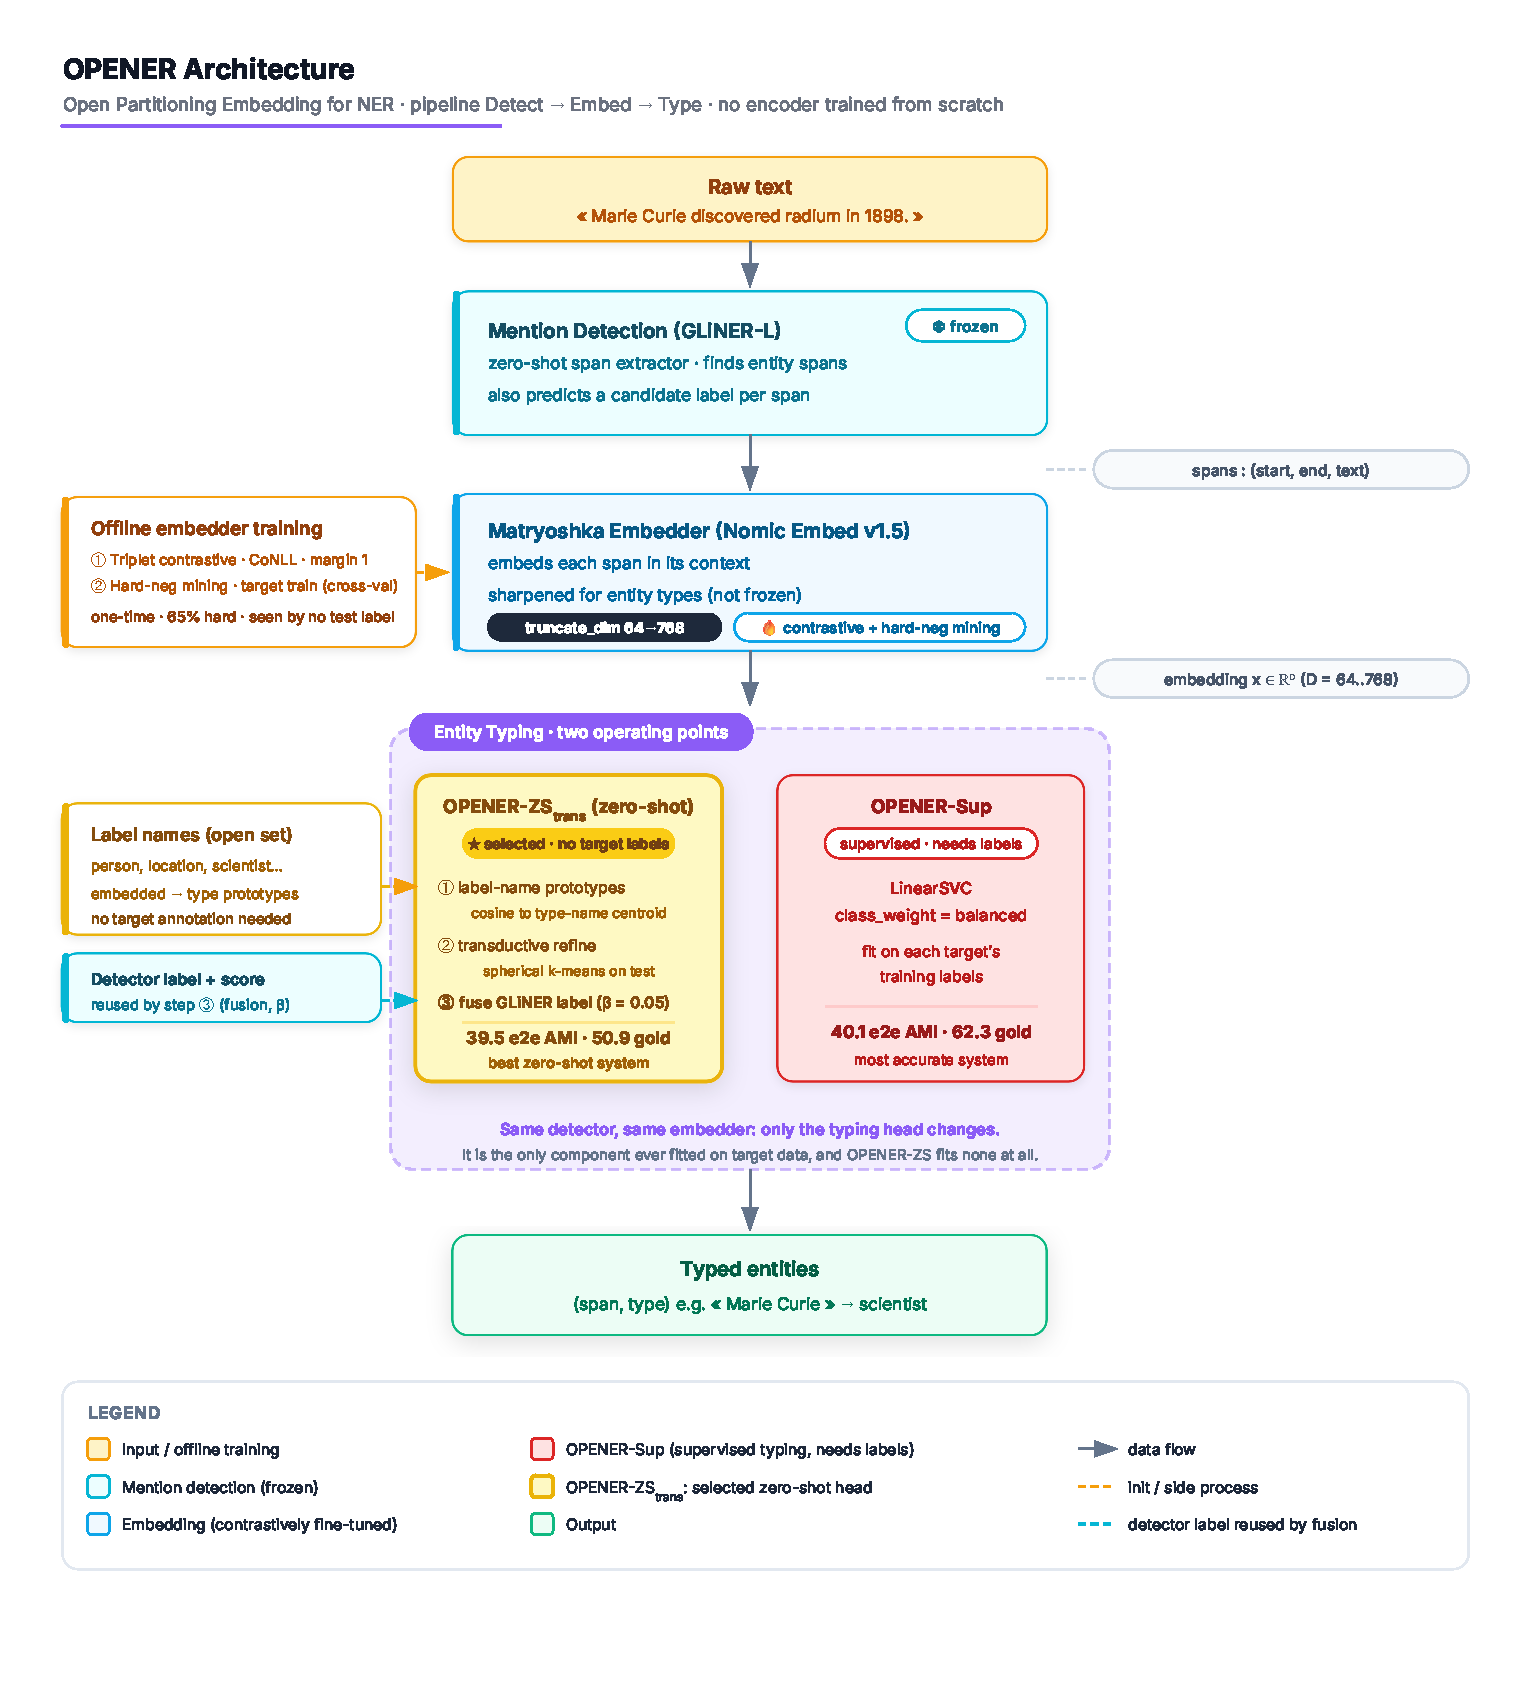
\includegraphics[width=0.82\linewidth]{Fig1}
\caption{The OPENER pipeline (Detect\,$\rightarrow$\,Embed\,$\rightarrow$\,Type): a frozen GLiNER detector proposes spans, a Matryoshka embedder (Nomic, contrastively fine-tuned) maps each span in context to a vector, and a typing head assigns a type. The typing head (the only target-fitted component) has two operating points: the \emph{zero-shot} \zstr ($\bigstar$, selected) and OPENER-Sup (\emph{supervised}, the upper bound). All upstream components are ready-to-use}
\label{fig:pipeline}
\end{figure*}

OPENER is a three-stage pipeline, Detect\,$\rightarrow$\,Embed\,$\rightarrow$\,Type (\autoref{fig:pipeline}), assembled from ready-to-use components so that no encoder is trained from scratch.
Three principles guide the design.
\begin{itemize}
\item A pretrained detector and a pretrained sentence embedder are reused as-is.
\item A light contrastive fine-tuning, refined by error-driven hard-negative mining, turns the general-purpose embedding into one that is discriminative for entity \emph{types}.
\item The embedder is Matryoshka-truncatable, exposing a compute/quality knob.
\end{itemize}
Only the typing head is fitted on target-side material, and it comes in two forms: a zero-shot form, OPENER-ZS, that uses no target labels at typing time and OPENER-Sup, a supervised linear probe that is the strongest configuration but requires target labels.

\subsection{Mention Detection}
\label{sec:method:detect}
Mention detection is delegated to GLiNER \cite{zaratiana2024gliner}, a frozen, ready-to-use detector that scores every span against the candidate type names in a single forward pass.
Decoupling detection from typing lets each component be chosen and measured independently, and it lets the typing head operate on any span proposer.
We use GLiNER-L by default, as it yields the best AMI. The small and medium variants trace a size/efficiency trade-off (see \autoref{tab:ablation} for the full detector comparison).
As shown in \autoref{sec:exp:results}, the detector is the shared end-to-end bottleneck: its recall on specialised domains, not the typing head, caps end-to-end quality.

\subsection{Entity Embedding}
\label{sec:method:embed}
Detected spans are embedded with Nomic Embed v1.5 \cite{nussbaum2024nomic}, a sentence embedder trained with the Matryoshka objective \cite{kusupati2022matryoshka}, whose representation can be truncated to a lower dimension and renormalised without retraining.
Each mention is embedded \emph{in context} rather than in isolation: the span is presented together with its surrounding sentence, so that polysemous surface forms (e.g.\ Apple as a company versus a fruit) are disambiguated.
This yields a vector $e_i \in \mathbb{R}^{D}$ with $D$ truncatable in $\{768,512,256,128,64\}$. We keep the full $D{=}768$, which gives the best AMI (see \autoref{tab:ablation} for the full dimension sweep).
Truncation keeps only the first $d$ coordinates of the embedding ($d \le D$) and rescales them back to unit length,
\begin{equation}
e_i^{(d)} = e_{i,1:d}\,\big/\,\lVert e_{i,1:d}\rVert_2 ,
\end{equation}
where $e_i \in \mathbb{R}^{D}$ is the in-context embedding of mention $m_i$, $e_{i,1:d}$ is its truncation to the first $d$ components (the coordinates $d{+}1$ to $D$ are simply dropped), and $\lVert e_{i,1:d}\rVert_2 = \sqrt{\sum_{k=1}^{d} e_{i,k}^2}$ is its Euclidean ($L_2$) norm, that is the geometric length of the vector. Dividing by this norm rescales $e_i^{(d)}$ to length $1$, so that embeddings truncated at different $d$ remain comparable through cosine similarity. This shrinks the stored embedding and the typing-head fit cost but leaves the forward pass unchanged (\autoref{tab:ablation}).

\label{sec:method:contrastive}
Still, the frozen embedding is only weakly discriminative for entity types ($25.8$ AMI, \autoref{tab:ablation}), so we sharpen its geometry with \emph{contrastive fine-tuning}, in two stages, while keeping the backbone otherwise intact.

\subsubsection{Stage 1: contrastive}
We fine-tune the embedder with a Triplet Margin Loss $\mathcal{L}$ \cite{schroff2015facenet} (using sentence-transformers \cite{reimers2019sbert}), with margin $\alpha = 1$, on the CoNLL-2003 \cite{tjongkimsang2003conll} training spans. We use CoNLL-2003 because its generic, domain-neutral label set makes it the standard source domain of our benchmark (\autoref{tab:datasets}). Since the embedder is only lightly fine-tuned on it, we exclude CoNLL-2003 from the reported average, so as not to bias the results in our favour, following the same protocol as OWNER.
A triplet $(a,p,n)$ takes an anchor span $a$, a positive $p$ of the \emph{same} type, and a negative $n$ of a \emph{different} type, with at most two triplets per anchor.
Writing $\alpha$ for the margin, each triplet contributes
% Layout only (two-column width): same equation as KBS, split on two lines.
\begin{equation}
\begin{split}
\mathcal{L}(a,p,n)&=\max\!\big(0,\;\lVert e_a-e_p\rVert_2-\lVert e_a-e_n\rVert_2+\alpha\big),\\
\alpha&=1,
\end{split}
\end{equation}
which pulls same-type spans together and pushes different-type spans apart, i.e.\ it decreases the embedding distance $\lVert e_a-e_p\rVert_2$ while increasing $\lVert e_a-e_n\rVert_2$.
Training runs for $3$ epochs with batch size $16$, learning rate $2\times10^{-5}$ and $100$ warmup steps.
This single step lifts typing-on-gold AMI from $25.8$ to $54.0$. The UMAP projection in \autoref{fig:umap} shows how Stage 1 reshapes the embedding space.

\begin{figure*}[!tp]
\centering
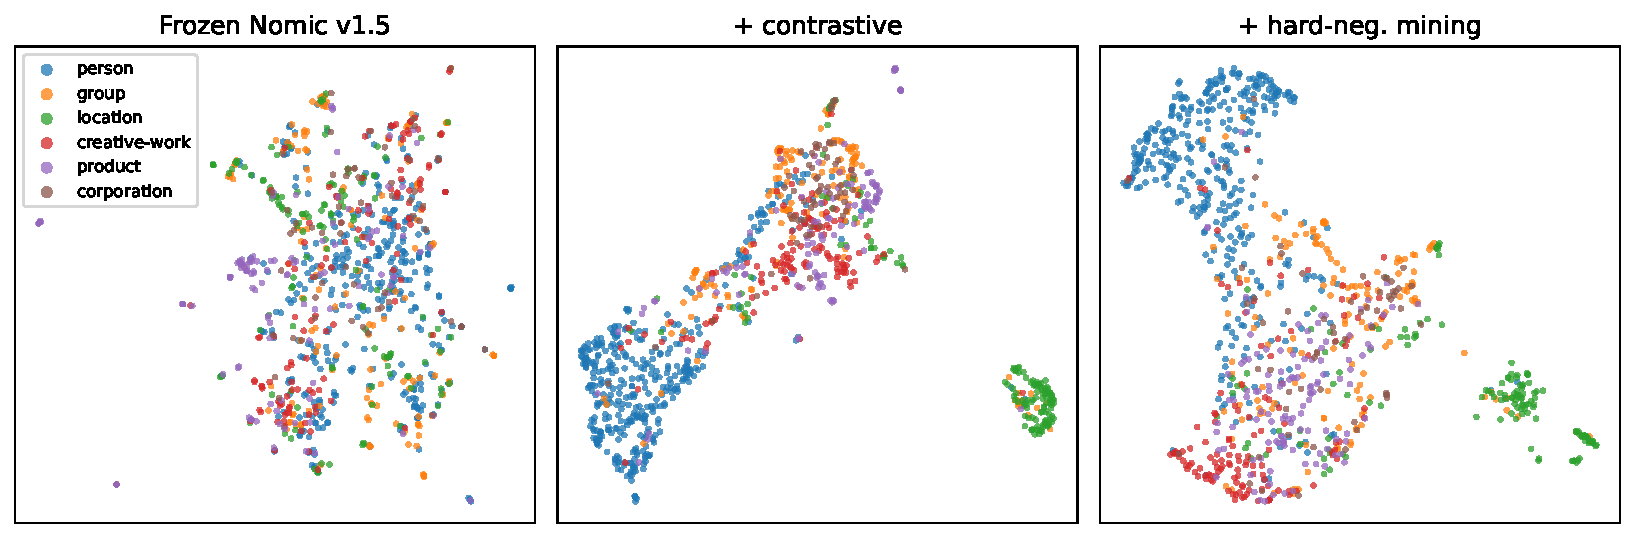
\includegraphics[width=\linewidth]{Fig2}
\caption{UMAP of WNUT-17 (held-out) entity embeddings, coloured by gold type, across the three embedder stages: frozen Nomic v1.5, $+$ contrastive fine-tuning, $+$ hard-negative mining. The contrastive stages progressively separate the types into compact clusters on a domain unseen during training}
\label{fig:umap}
\end{figure*}


\subsubsection{Stage 2: error-driven hard-negative mining}
We then mine the model's own confusions. We defer this to Stage 2, after the Stage-1 warm-up, to avoid overfitting to these hard cases.
On each target training split, we run a cross-validated typing pass (so no test label is ever seen) and collect the type pairs that are most often confused, such as \emph{writer}/\emph{person}, \emph{album}/\emph{band} and \emph{country}/\emph{location}.
For each such error, we form a \emph{hard} triplet whose anchor is the mistyped span (true type $L$), whose positive is another span of $L$, and whose negative is a span of the confused type $C$.
Hard triplets are mixed with correctly-typed (easy) triplets for diversity, targeting a $65\%$ hard fraction, and the Stage-1 embedder is fine-tuned further with the same optimiser settings. This ratio must be controlled carefully to preserve generalisation.
The selected run mines $8000$ triplets over $3$ epochs and reaches $62.5$ AMI at the released seed ($+8.5$ over Stage~1, improving on $12$ of the $13$ sets). Retraining the full two-stage recipe under three seeds yields $62.3 \pm 1.0$ (\autoref{sec:exp:protocol}).
This embedder is shared unchanged by every typing head below. The UMAP projection in \autoref{fig:umap} also reveals the additional effect of Stage 2 on the embedding space.

\subsection{Entity Typing}
\label{sec:method:typing}

The embedding above feeds a typing head, the only component fitted on target-side material. It has two operating points, presented in turn: a label-free \emph{zero-shot} head, OPENER-ZS, which we adopt as the open-world default, and a \emph{supervised} probe, OPENER-Sup, a stronger but label-dependent upper bound.

\subsubsection{Zero-shot typing (OPENER-ZS)}
To remove target supervision at typing time, each type $t$ is represented by a prototype $p_t$: the $\ell_2$-normalised centroid of the embeddings of its name (its anchor words) in the contrastive space,
\begin{equation}
p_t = \overline{e}_t\,\big/\,\lVert \overline{e}_t\rVert_2,\qquad \overline{e}_t=\frac{1}{|\mathrm{name}(t)|}\!\!\sum_{w\,\in\,\mathrm{name}(t)}\!\!f_\theta(w),
\end{equation}
where $t$ is a candidate type, $\mathrm{name}(t)$ is the set of words forming its name (its anchor words, e.g.\ ``person'' or ``astronomical object''), $f_\theta(w)$ is the embedding of anchor word $w$ in the contrastive space, and $\overline{e}_t$ is their average (the centroid), which dividing by its Euclidean norm $\lVert\overline{e}_t\rVert_2$ turns into a unit-length prototype $p_t$ (the averaging factor cancels under this normalisation). A mention $m_i$ is then assigned the type of the nearest prototype by cosine similarity, $\hat y_i = \arg\max_t \cos(e_i, p_t)$. This inductive nearest-centroid head is \zsind.
Two label-free refinements improve this head without using any target label.
First, a \emph{transductive} refinement runs one pass of spherical $k$-means over the unlabelled test mentions, seeded by the prototypes.
Second, a \emph{detector fusion} reuses a signal the prototype head otherwise discards: GLiNER already predicts a zero-shot type for each span with confidence $g_i$, which we add to the similarity score before taking the arg-max,
\begin{equation}
s_t(i)=\cos(e_i,p_t)+\beta\,g_i\,\mathbb{1}\!\left[t=\ell_{\text{GLiNER}}(i)\right],
\end{equation}
where $s_t(i)$ is the fused score of assigning type $t$ to mention $m_i$, $\cos(e_i,p_t)$ is the prototype similarity above, $g_i\in[0,1]$ is GLiNER's own confidence for the type $\ell_{\text{GLiNER}}(i)$ it predicted, and $\mathbb{1}[\cdot]$ is the indicator function, equal to $1$ when $t$ is exactly that predicted type and $0$ otherwise. The fusion weight $\beta{=}0.05$ was found by a small empirical sweep and is deliberately kept low, so the detector only nudges the arg-max, and the assigned type is the highest-scoring one, $\hat y_i=\arg\max_t s_t(i)$.
The refined, fused head is \zstr, the selected zero-shot operating point: it reaches $39.5$ AMI end-to-end (mean over three retraining seeds), ahead of every compared zero-shot system, while using no target labels (\autoref{sec:exp:results}).

\subsubsection{Supervised probe (OPENER-Sup)}
When a domain's entity classes are fixed and labelled, the typing head can instead be a balanced linear classifier (LinearSVC with the LIBLINEAR solver \cite{fan2008liblinear}) fitted one-vs-rest on the target's training labels.
For each type $c$, it minimises a squared-hinge objective with balanced class weights,
% Layout only (two-column width): same equation as KBS, split on two lines.
\begin{equation}
\begin{split}
\min_{w_c,b_c}\;&\tfrac12\lVert w_c\rVert_2^2\\
&+C\sum_i \omega_{y_i}\,\max\!\big(0,\,1-z_{ic}(w_c^{\top} e_i+b_c)\big)^2,
\end{split}
\end{equation}
where, for each type $c$, $w_c$ and $b_c$ are the weight vector and bias of its one-vs-rest hyperplane, $e_i$ is the (frozen) embedding of training mention $i$ and $y_i$ its gold type, $z_{ic}{=}{+}1$ if $y_i{=}c$ and ${-}1$ otherwise, and $C$ is the regularisation strength that trades margin width against training errors. The squared-hinge term $\max(0,\,1-z_{ic}(w_c^{\top}e_i+b_c))^2$ penalises mentions on the wrong side of the margin. The balancing weight $\omega_c=n/(|\mathcal{T}|\,n_c)$, with $n$ the total number of training mentions, $|\mathcal{T}|$ the number of target types and $n_c$ the count of type $c$, up-weights rare types to counter the benchmark's heavy imbalance. A mention is finally typed as $\hat y_i=\arg\max_c (w_c^{\top}e_i+b_c)$.
This is the strongest configuration but requires target-side labels.

\subsection{Evaluation Protocol}
\label{sec:method:eval}
We evaluate on the $13$ datasets of \autoref{sec:exp:datasets}, each test split capped at $1000$ sentences.
Quality is AMI \cite{vinh2010ami} (with macro-$F_1$ and accuracy), latency is the median (p50) per-sentence time over GPU-synchronised, warmed-up passes, and energy is measured with CodeCarbon \cite{luccioni2019quantifying} under the French grid carbon intensity. The full protocol and instrumentation are detailed in \autoref{sec:exp:protocol} and \autoref{sec:exp:impl}.
The code and the per-experiment configurations are available on GitHub at \url{https://github.com/Thibault-GAREL/LyRIDS_OPENER}, and the fine-tuned embedders of OPENER-ZS and OPENER-Sup are available on Hugging Face at \url{https://huggingface.co/Thibault-GAREL/opener-zs} and \url{https://huggingface.co/Thibault-GAREL/opener-sup}, respectively.

% JIIS (Springer Nature): "Use of an LLM should be properly documented in the
% Methods section". Text moved here from the KBS generative-AI declaration.
\subsection{Use of Generative AI Tools}
\label{sec:method:genai}
During the preparation of this work the first author used Claude Code (Anthropic) in order to scaffold and debug the experiment scripts, to draft and copy-edit the manuscript, and to assist with exploratory data analysis.
The research questions, the experimental design, the choice of baselines and datasets, the execution of all experiments, and the interpretation of the results are the first author's own.
After using this tool, the authors reviewed and edited the content as needed and take full responsibility for the content of the published article.

\section{Experiments}
\label{sec:experiments}

\subsection{Datasets}
\label{sec:exp:datasets}

\begin{table*}[!t]
\centering
\caption{The 13 evaluation sets and their gold entity types.}
\label{tab:datasets}
\scriptsize
\setlength{\tabcolsep}{4pt}
\begin{adjustbox}{max width=\textwidth}
\begin{threeparttable}
% p column widened from 0.40 to 0.52\linewidth: fewer wrapped lines per cell,
% so the table fits the page height; the enclosing adjustbox absorbs the
% extra natural width (KBS/elsarticle 12pt text width is narrower than IEEE).
\begin{tabular}{@{}lllr>{\raggedright\arraybackslash}p{0.52\linewidth}@{}}
\toprule
Dataset & Abbr. & Domain & Test & Entity types (share \%) \\
\midrule
CrossNER-AI & AI & encyclopaedic (AI) & 430 & task 12, field 11, product 11, metrics 11, misc 10, algorithm 10, researcher 9, organisation 8, conference 5, person 4, programlang 3, country 2, location 2, university 2 \\
\addlinespace
CrossNER-Literature & Lit & encyclopaedic (literature) & 416 & writer 25, book 18, misc 11, literarygenre 9, person 8, award 6, poem 5, organisation 5, country 4, location 4, magazine 3, event 2 \\
\addlinespace
CrossNER-Music & Mus & encyclopaedic (music) & 465 & musicalartist 15, musicgenre 15, band 14, location 10, album 10, award 8, song 7, organisation 6, misc 5, country 5, person 2, event 2, musicalinstrument 1 \\
\addlinespace
CrossNER-Politics & Pol & encyclopaedic (politics) & 651 & politicalparty 23, location 14, organisation 12, politician 12, election 10, country 10, person 8, misc 6, event 5 \\
\addlinespace
CrossNER-Science & Sci & encyclopaedic (science) & 543 & misc 17, scientist 15, astronomicalobject 11, organisation 9, person 7, academicjournal 6, location 6, chemicalcompound 5, protein 5, award 5, university 4, chemicalelement 3, enzyme 3, discipline 2, event 1, country 1, theory 1 \\
\addlinespace
WNUT-17 & WNUT & Social media & 689 & person 40, group 15, location 14, creative-work 13, product 12, corporation 6 \\
\addlinespace
MIT-Restaurant & Rest & Restaurant search & 1000 & Location 21, Dish 18, Amenity 16, Hours 15, Restaurant\_Name 11, Price 10, Cuisine 5, Rating 4 \\
\addlinespace
MIT-Movie & Movie & Movie trivia & 1000 & TITLE 19, ACTOR 16, YEAR 16, GENRE 16, RATING 9, CHARACTER 9, TRAILER 5, REVIEW 3, RATINGS\_AVERAGE 3, PLOT 2, DIRECTOR 2, SONG 1 \\
\addlinespace
FabNER & Fab & Manufacturing & 1000 & MATE 27, CONPRI 21, MANP 15, PRO 11, APPL 6, FEAT 6, PARA 4, MACEQ 3, BIOP 2, CHAR 2, ENAT 2, MANS $<$1 \\
\addlinespace
BioNLP/JNLPBA-2004 & Bio & Biomedical & 1000 & protein 53, cell\_type 22, DNA 13, cell\_line 10, RNA 1 \\
\addlinespace
CoNLL-2003 & CoNLL & News & 1000 & PER 32, ORG 29, LOC 28, MISC 11 \\
\addlinespace
GUM & GUM & Multi-genre & 1000 & abstract 38, person 17, event 12, place 10, object 8, organization 8, time 5, substance 1, animal 1, plant $<$1 \\
\addlinespace
GENTLE & GEN & Multi-genre (challenge) & 1000 & abstract 55, person 10, event 9, time 8, object 7, place 5, organization 4, animal 1, substance 1, plant $<$1 \\
\bottomrule
\end{tabular}
\begin{tablenotes}[flushleft]
\footnotesize
\item ``Test'' column is the number of test sentences used (capped at 1000). Each type is followed by its share (\%) of the test mentions, listed by decreasing frequency (types are the dataset's original labels).
\end{tablenotes}
\end{threeparttable}
\end{adjustbox}
\end{table*}

We evaluate on 13 evaluation sets that span news, social media, spoken queries, encyclopaedic text, biomedical abstracts and manufacturing literature, following the dataset selection of OWNER \cite{genest2025owner}.
CrossNER \cite{liu2021crossner} contributes five domain-specific sets, evaluated separately (artificial intelligence, literature, music, politics, science).
The remaining eight are CoNLL-2003 \cite{tjongkimsang2003conll}, WNUT-17 \cite{derczynski2017wnut}, the MIT-Restaurant and MIT-Movie spoken-query corpora \cite{liu2013asgard}, FabNER \cite{kumar2022fabner}, the BioNLP/JNLPBA-2004 biomedical task \cite{kim2004jnlpba}, and the GUM \cite{zeldes2017gum} and GENTLE \cite{aoyama2023gentle} multi-genre corpora.
Label granularity ranges from four coarse types in CoNLL-2003 to seventeen fine-grained categories in CrossNER-Science, including the opaque domain acronyms of FabNER.
Two datasets used by OWNER \cite{genest2025owner}, GENIA \cite{kim2003genia} and the 2014 i2b2\slash UTHealth clinical corpus, are license-gated and therefore not re-measured here. BioNLP/JNLPBA-2004 serves as our biomedical proxy.
To homogenise evaluation cost across systems, we cap each test split at $1000$ sentences (the full split is used when it is smaller).

\subsection{Baselines}
\label{sec:exp:baselines}

\begin{table*}[!t]
\centering
\caption{Backbones and size of the re-measured baselines and OPENER, in the spirit of OWNER \cite{genest2025owner}.}
\label{tab:baselines}
\footnotesize
\setlength{\tabcolsep}{4.5pt}
\begin{adjustbox}{max width=\textwidth}
\begin{threeparttable}
\begin{tabular}{@{}llllrr@{}}
\toprule
Model & Backbone & Type & Version & Params & vs OPENER \\
\midrule
GLiNER-S & DeBERTaV3 & Encoder & deberta-v3-small & 50M & 0.1$\times$ \\
GLiNER-M & DeBERTaV3 & Encoder & deberta-v3-base & 200M & 0.4$\times$ \\
GLiNER-L & DeBERTaV3 & Encoder & deberta-v3-large & 330M & 0.7$\times$ \\
GNER & T5 & Enc.-Dec. & t5-base & 220M & 0.5$\times$ \\
OWNER\tnote{a} & DeBERTaV3+BERT & Encoder & deberta-v3 + bert-base & 294M & 0.6$\times$ \\
Qwen2.5-1.5B & Qwen2.5 & Decoder & qwen2.5-1.5b-instruct & 1.5B & 3.2$\times$ \\
\midrule
\rowcolor{hlorange} \textbf{OPENER} (ours) & DeBERTaV3+Nomic & Encoder & deberta-v3-large + nomic-v1.5 & 467M & 1.0$\times$ \\
\bottomrule
\end{tabular}
\begin{tablenotes}[flushleft]
\footnotesize
\item ``Type'' column is the transformer family. ``vs OPENER'' column is the total parameter count relative to OPENER's end-to-end pipeline ($467$M $=$ GLiNER-L $330$M detector $+$ Nomic $137$M embedder).
\item[a] OWNER reports $110$M for its BERT typing encoder. We count detection $+$ typing for parity with OPENER.
\end{tablenotes}
\end{threeparttable}
\end{adjustbox}
\end{table*}

We compare OPENER with representative open-world systems, all run end-to-end on the same splits and scored with the same protocol (\autoref{sec:exp:protocol}). \autoref{tab:baselines} summarises their backbones and sizes.
\begin{itemize}
\item \textbf{GLiNER} \cite{zaratiana2024gliner}: an open-world span classifier that scores every candidate span against the supplied type names in a single forward pass on a DeBERTaV3 encoder \cite{he2023debertav3}. It is a strong and fast detector, but its predicted types are limited to the names given as queries. We run all three sizes (S/M/L) to trace a size/efficiency trade-off.
\item \textbf{GNER} \cite{ding2024gner}: a generative tagger built on T5 \cite{raffel2020t5} that regenerates the sentence with inline type tags. It is accurate, but its autoregressive decoding makes inference really slower than the encoder-based detectors. We run the T5-base checkpoint.
\item \textbf{OWNER} \cite{genest2025owner}: our closest baseline, a DeBERTaV3 detector with a BERT typing encoder \cite{devlin2019bert} refined by contrastive learning, whose mentions are grouped into dynamically named types by a plain unsupervised $k$-means. This keeps it fully label-free, but it re-encodes and re-clusters every mention at inference time, which is costly. We execute it in its original environment.
\item \textbf{Qwen2.5-1.5B-Instruct} \cite{qwen2025}: the only generative LLM that fits our $6$\,GB GPU, runs in 4-bit NF4 \cite{dettmers2023qlora} and prompted for JSON-formatted entities. Even at this small size, its autoregressive decoding makes it the slowest system we measure and, per sentence, the most energy-hungry, showing that generative extraction remains costly regardless of model size.
\item \textbf{Large LLM systems}: UniversalNER \cite{zhou2024universalner}, GoLLIE \cite{sainz2024gollie} and ChatIE \cite{wei2024chatie} reach strong accuracy but rely on $7$B-parameter backbones \cite{touvron2023llama} whose compute and energy cost is far higher and which exceed our hardware even under 4-bit quantisation. We therefore discuss them qualitatively and omit them from \autoref{tab:baselines} and the measured comparison. For LLM extraction figures under a comparable AMI protocol, we refer the reader to the benchmark of OWNER \cite{genest2025owner}, whose findings are consistent with our, measurements.
\end{itemize}

\subsection{Metrics}
\label{sec:exp:metrics}
Our primary metric is the Adjusted Mutual Information (AMI) \cite{vinh2010ami} between predicted and gold type assignments, following OWNER \cite{genest2025owner}, complemented by macro-averaged $F_1$ and accuracy.
Because open-world predictions need not share the gold label vocabulary, AMI is computed over the aligned set of mentions, which makes it well suited to comparing dynamically named types.
Beyond quality, we report two efficiency axes: inference \emph{speed}, as the median (p50) latency per sentence, and \emph{energy}, as kilowatt-hours and grams of CO\textsubscript{2}eq per run.

\subsection{Evaluation Protocol}
\label{sec:exp:protocol}
The predicted and gold mentions are aligned by exact character offsets, and any unmatched mention receives a distinct sentinel label so that detection errors are penalised rather than ignored, following the sentinel-based scoring detailed in \autoref{sec:method:problem}.
We distinguish two protocols that must not be mixed in the same comparison.
In the \emph{typing-on-gold} protocol, the entity-typing component is applied to gold mention spans, which measures typing quality in isolation under perfect detection.
In the \emph{end-to-end} protocol, the detector produces mentions and the sentinel labels above are active, which is a setting comparable to the baselines.
OPENER's embedder \emph{training} is stochastic (triplet sampling and optimisation), so we retrain the complete embedder (contrastive Stage~1, then hard-negative mining Stage~2) under three random seeds ($7$, $42$, $123$) and re-evaluate every OPENER operating point on the full benchmark with each resulting embedder.
Therefore, every OPENER cell in the result tables reports the mean\,$\pm$\,standard deviation over the three seeds. Seed $42$ is the model released.
The compared baselines are frozen pretrained checkpoints whose inference is deterministic, so re-running them under a different seed returns identical predictions and they are reported as single runs. OWNER, the only baseline that trains, is likewise reported from a single training run of its published protocol.
We also quantify the test-set sampling uncertainty with a bootstrap on the released model (\autoref{tab:bootstrap}), a source of uncertainty orthogonal to the retraining seed.

\subsection{Experimental Settings}
\label{sec:exp:impl}
% Tables 3 and 4 are declared at the start of this subsection (not after its text), so they
% do not pile up with Tables 1-2 nor delay Table 5 / Fig. 3.
\begin{table*}[!t]
\centering
\caption{Test-set bootstrap robustness of the released (seed-$42$) model on three representative datasets.}
\label{tab:bootstrap}
\small
\begin{adjustbox}{max width=\textwidth}
\begin{threeparttable}
\begin{tabular}{lccc}
\toprule
Model & CoNLL-2003 & CrossNER-Music & FabNER \\
\midrule
\zsind{}   & $66.1 \pm 1.4$ ~[$63.5$, $69.0$] & $55.5 \pm 0.9$ ~[$53.8$, $57.3$] & $36.2 \pm 0.7$ ~[$34.7$, $37.5$] \\
OPENER-Sup & $71.7 \pm 1.5$ ~[$68.9$, $74.6$] & $72.4 \pm 0.9$ ~[$70.6$, $74.2$] & $59.8 \pm 0.9$ ~[$57.9$, $61.6$] \\
\bottomrule
\end{tabular}
\begin{tablenotes}[flushleft]
\footnotesize
\item Typing-on-gold AMI ($\uparrow$) as bootstrap mean $\pm$ std [$95\%$ percentile CI], over $K{=}1000$ resamples of the gold mentions. The transductive refinement is excluded, as it adapts to the resampled test distribution. The bootstrap means match the full-test-set scores, and the stds stay at or below $1.5$ AMI, indicating stable scores.
\end{tablenotes}
\end{threeparttable}
\end{adjustbox}
\end{table*}
\begin{table*}[!t]
\centering
\caption{OPENER configuration.}
\label{tab:hyperparams}
\small
\begin{adjustbox}{max width=\textwidth}
\begin{threeparttable}
\begin{tabular}{ll}
\toprule
Component & Setting \\
\midrule
Mention detector   & GLiNER-L (frozen) \cite{zaratiana2024gliner} \\
Entity embedder    & Nomic v1.5, $D{=}768$, span-in-context \cite{nussbaum2024nomic} \\
Contrastive loss   & Triplet margin $1$ \cite{schroff2015facenet} \\
\quad source        & CoNLL-2003 train spans \cite{tjongkimsang2003conll} \\
\quad optimiser     & $3$ epochs, batch $16$, lr $2\times10^{-5}$, $100$ warmup \\
Hard-neg.\ mining  & $8000$ triplets, $65\%$ hard, $3$ epochs \\
\quad source        & target train splits, cross-validated \\
Supervised typing  & LinearSVC, balanced weights \cite{fan2008liblinear} \\
Zero-shot typing   & label-name prototype $+$ transductive $+$ fusion ($\beta{=}0.05$) \\
Random seeds       & $7$ / $42$ / $123$ (full embedder retraining per seed, $42$ = released) \\
\bottomrule
\end{tabular}
\begin{tablenotes}[flushleft]
\footnotesize
\item The detector and embedder are ready-to-use. The contrastive and hard-mining stages produce the shared embedder. The typing head is fitted (supervised) or label-free (zero-shot).
\end{tablenotes}
\end{threeparttable}
\end{adjustbox}
\end{table*}
All experiments run on a single consumer-grade GPU, an NVIDIA GeForce GTX 1660 Ti Max-Q with $6$\,GB of VRAM (CUDA~12.1, PyTorch~2.5.1 \cite{paszke2019pytorch}). The goal of using such modest hardware was to verify that the models could also run on standard personal computers, demonstrating that our approach is highly versatile.
We use the HuggingFace Transformers library \cite{wolf2020transformers} for baselines, sentence-transformers \cite{reimers2019sbert} for the Matryoshka embedder \cite{nussbaum2024nomic, kusupati2022matryoshka}, and scikit-learn \cite{pedregosa2011scikit} for the linear classifier, whose solver is LIBLINEAR \cite{fan2008liblinear}.
Latency is measured with two warmup passes followed by timed passes with GPU synchronisation, reporting p50, p95 and p99 per sentence.
Energy is measured with CodeCarbon \cite{luccioni2019quantifying} in offline mode using the French grid carbon intensity. When hardware power counters are unavailable, we fall back to a thermal-design-power estimate and flag the measurement method in the report.
All systems are measured on the same machine. Our consumer GPU is subject to \emph{thermal throttling} (it lowers its clock frequency under sustained load to stay within its temperature limit), so per-sentence latency and per-run energy carry roughly $\pm15\%$ run-to-run variance. Therefore, we read the per-system averages as indicative and do not over-interpret individual per-dataset cells.
The quality metrics, in contrast, are fully deterministic: with the fixed seed and the released model, no stage of the OPENER pipeline is stochastic at inference, so its AMI and $F_1$ reproduce exactly across re-runs (we verified identical CrossNER scores on an independent re-run), and only latency and energy fluctuate.
Because inference is deterministic, the only remaining source of uncertainty in quality scores is the finite test set. We quantify it with a non-parametric bootstrap: for three representative datasets, we resample the gold mentions with replacement ($K{=}1000$ resamples) and recompute typing-on-gold AMI, yielding the $95\%$ confidence intervals in \autoref{tab:bootstrap}. The uncertainty is small (bootstrap std of at most $1.5$ AMI, $95\%$ CIs within roughly $\pm 3$ AMI) and the bootstrap means coincide with the released model's full-test-set scores, indicating that the reported figures are stable rather than fragile seed-specific artefacts.
\autoref{tab:hyperparams} collects the complete OPENER configuration used throughout. The embedder is retrained under each of the three seeds ($7$, $42$, $123$) while every other component is fixed.



\subsection{Main Results}
\label{sec:exp:results}
% OPENER numbers = mean±std over seeds 7/42/123, from
% outputs/results/aggregate/results_multiseed.json (scripts/aggregate_multiseed.py,
% 2026-07-08); baseline numbers from results_all.json (2026-06-12).
% OWNER in its native zero-shot transfer protocol (train once on CoNLL-2003,
% infer on every target). $\S$ = zero-shot transfer; $\dagger$ = in-domain (CoNLL source).
The tables below report the benchmark on all $13$ sets, and \autoref{fig:main} plots the per-dataset end-to-end AMI of every system.

% --- Float page A: Table 5, Fig. 3, Table 6 (one float, no text in between)
\begin{table*}[p]
\centering
\caption{Open-world NER, end-to-end. AMI ($\times 100$, $\uparrow$).}
\label{tab:main}
\scriptsize
\setlength{\tabcolsep}{2.5pt}
\begin{adjustbox}{max width=\textwidth}
\begin{threeparttable}
\begin{tabular}{l*{13}{c}c}
\toprule
Model & AI & Lit & Mus & Pol & Sci & WNUT & Rest & Movie & Fab & Bio & CoNLL & GUM & GEN & Avg \\
\midrule
\multicolumn{15}{l}{\emph{Zero-shot (no target labels)}} \\
GLiNER-S & 41.7 & 49.8 & 56.4 & 50.6 & 53.3 & 29.7 & 26.1 & 35.6 & 10.7 & 31.8 & 18.9 & \textbf{34.1} & \textbf{36.1} & 36.5 \\
GLiNER-M & 42.0 & \textbf{50.1} & 57.4 & 50.2 & \textbf{54.2} & 28.1 & 27.9 & 36.4 & 11.3 & 34.9 & 24.9 & 32.8 & 31.6 & 37.1 \\
GLiNER-L & 42.9 & 48.9 & 58.0 & 49.8 & 52.8 & 28.9 & 30.9 & 37.6 & 28.1 & 34.6 & 29.7 & 32.7 & 30.5 & 38.9 \\
GNER & 41.9 & 46.9 & 53.5 & 48.9 & 49.9 & \textbf{30.0} & 30.0 & 36.8 & 17.0 & 29.1 & \textbf{43.7} & 32.8 & 31.6 & 37.9 \\
Qwen2.5-1.5B\textsuperscript{b} & 25.4 & 30.5 & 30.5 & 28.3 & 34.1 & 27.8 & 5.0 & 27.4 & 12.9 & 29.9 & 15.5 & 37.2 & 34.6 & 26.1 \\
OWNER & \textbf{43.9} & 44.0 & 46.6 & \textbf{50.9} & 50.3 & 22.3 & 7.6 & 24.0 & 18.7 & 26.5 & 50.3\textsuperscript{a} & 29.1 & 31.3 & 34.3 \\
% Multi-seed (7/42/123, mean±std). NB: la ligne \zsind suit desormais le protocole
% "fusion beta=0" (inductif pur du run fusion), coherent seed a seed ; l'ancien run
% separe opener_zs_e2e (seed 42 : 31.6 43.8 41.7 ... | 34.2) est conserve ici.
\zsind & 29.7$_{\pm2.2}$ & 41.6$_{\pm2.3}$ & 43.6$_{\pm0.3}$ & 40.4$_{\pm0.7}$ & 42.5$_{\pm0.6}$ & 21.9$_{\pm1.3}$ & 28.0$_{\pm1.9}$ & 32.8$_{\pm0.9}$ & 27.6$_{\pm0.1}$ & 26.2$_{\pm1.4}$ & 43.5$_{\pm1.6}^{\text{a}}$ & 30.8$_{\pm1.4}$ & 30.1$_{\pm1.0}$ & 33.8$_{\pm0.7}$ \\
\rowcolor{hlyellow} \zstr & 39.4$_{\pm2.1}$ & 48.7$_{\pm0.7}$ & \textbf{58.3$_{\pm0.3}$} & 49.2$_{\pm0.9}$ & 52.6$_{\pm0.2}$ & 28.8$_{\pm1.0}$ & 31.2$_{\pm0.2}$ & 36.0$_{\pm0.6}$ & 28.1$_{\pm0.3}$ & 34.7$_{\pm0.9}$ & 43.7$_{\pm1.1}^{\text{a}}$ & 32.0$_{\pm0.7}$ & 30.7$_{\pm0.3}$ & 39.5$_{\pm0.1}$ \\
%       --       MOVED to architecture search (\autoref{tab:ablation}); preserved e2e per-dataset:
% OPENER-ZS (transd.) & 33.7 & 48.9 & 53.7 & 45.3 & 45.9 & 24.2 & 30.4 & 34.7 & 27.9 & 27.9 & 44.4\textsuperscript{a} & 31.0 & 30.8 & 36.8 \\
\addlinespace
\multicolumn{15}{l}{\emph{Supervised (target labels)}} \\
%       --       DATA PRESERVED (pre-hard-mining OPENER e2e, contrastive only, 2026-06-09)       --
% OPENER & 39.1 & 39.3 & 49.2 & 44.2 & 47.8 & 24.8 & 30.6 & 36.7 & \textbf{28.3} & 31.4 & 39.4 & 32.5 & 32.5 & 36.6 \\
%       --       end preserved       --
% hard-mining 3k tr./2 ep. e2e (recorded in project notes): 41.0 47.0 53.3 48.3 50.0 24.0 33.1 37.3 30.1 33.5 45.6 33.2 33.9 | 39.2
\rowcolor{hlred} OPENER-Sup & 40.3$_{\pm0.2}$ & 48.7$_{\pm1.3}$ & 55.2$_{\pm0.8}$ & 49.1$_{\pm1.4}$ & 51.8$_{\pm1.7}$ & 24.8$_{\pm0.2}$ & \textbf{34.1$_{\pm0.9}$} & \textbf{37.8$_{\pm0.2}$} & \textbf{29.8$_{\pm0.5}$} & \textbf{35.9$_{\pm0.5}$} & 46.1$_{\pm2.1}^{\text{a}}$ & 33.8$_{\pm0.1}$ & 34.0$_{\pm0.3}$ & \textbf{40.1$_{\pm0.5}$} \\
\bottomrule
\end{tabular}
\begin{tablenotes}[flushleft]
\footnotesize
\item Abbreviations follow \autoref{tab:datasets}. Bold marks the best value per column across all systems. Systems are grouped by supervision (\emph{zero-shot} vs the \emph{supervised} OPENER-Sup). OPENER rows report mean\,$\pm$\,std over the three embedder-retraining seeds (\autoref{sec:exp:protocol}). The baselines are frozen checkpoints with deterministic inference (single run). Typing-on-gold is reported in \autoref{tab:et-gold}.
\item[a] CoNLL-2003 is in-domain for OWNER (training source) and OPENER (contrastive source) and is not bolded as a transfer result.
\item[b] Qwen2.5-1.5B-Instruct (4-bit) is on a $150$-sentence subsample (indicative).
\end{tablenotes}
\end{threeparttable}
\end{adjustbox}
\par\bigskip
\figurecaptype
\centering
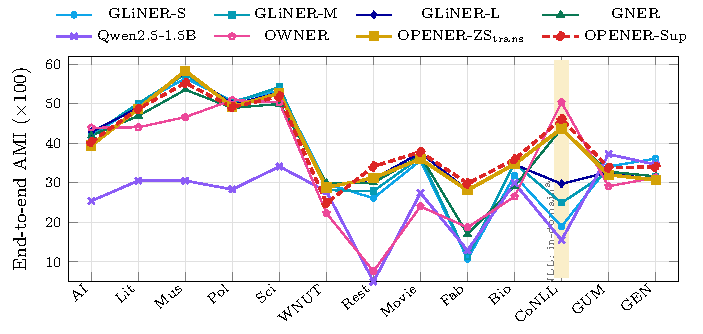
\includegraphics{Fig3}
\caption{End-to-end AMI per dataset (\autoref{tab:main}, OPENER curves show the three-seed means). \emph{Zero-shot} systems are drawn solid. OPENER-Sup is the dashed red line. \textsuperscript{a}\,CoNLL-2003 (shaded) is in-domain for OWNER and OPENER. \textsuperscript{b}\,Qwen is evaluated on a $150$-sentence subsample per set}
\label{fig:main}
\par\bigskip
\tablecaptype
\centering
\caption{Median per-sentence latency (ms, $\downarrow$), end-to-end.}
\label{tab:latency}
\footnotesize
\setlength{\tabcolsep}{4pt}
\begin{adjustbox}{max width=\textwidth}
\begin{threeparttable}
\begin{tabular}{l*{13}{c}c}
\toprule
Model & AI & Lit & Mus & Pol & Sci & WNUT & Rest & Movie & Fab & Bio & CoNLL & GUM & GEN & Avg \\
\midrule
\multicolumn{15}{l}{\emph{Zero-shot (no target labels)}} \\
GLiNER-S & \textbf{21} & \textbf{22} & \textbf{21} & \textbf{21} & \textbf{21} & \textbf{20} & \textbf{19} & \textbf{20} & \textbf{20} & \textbf{22} & \textbf{20} & \textbf{21} & \textbf{21} & \textbf{21} \\
GLiNER-M & 36 & 36 & 37 & 38 & 39 & 39 & 38 & 40 & 41 & 42 & 44 & 46 & 45 & 40 \\
GLiNER-L & 144 & 149 & 153 & 149 & 155 & 137 & 132 & 145 & 147 & 143 & 131 & 141 & 137 & 143 \\
GNER & 3431 & 5408 & 7461 & 6472 & 7110 & 2906 & 1610 & 3344 & 4310 & 5034 & 2914 & 3435 & 1500 & 4226 \\
Qwen2.5-1.5B\textsuperscript{b} & 4857 & 6757 & 9396 & 7700 & 8261 & 3553 & 2142 & 5014 & 2921 & 4737 & 2260 & 4265 & 3806 & 5051 \\
OWNER\textsuperscript{c} & 500 & 712 & 895 & 920 & 757 & 311 & 281 & 532 & 438 & 558 & 719\textsuperscript{a} & 759 & 626 & 616 \\
\zsind & 109 & 135 & 156 & 172 & 175 & 136 & 127 & 137 & 133 & 136 & 117 & 127 & 124 & 137 \\
\rowcolor{hlyellow} \zstr & 218 & 254 & 291 & 277 & 289 & 185 & 173 & 205 & 84 & 98 & 92 & 104 & 97 & 182 \\
% MOVED to architecture search (\autoref{tab:ablation}); preserved e2e per-dataset:
% OPENER-ZS (transd.) & 104 & 130 & 149 & 158 & 186 & 186 & 217 & 233 & 194 & 132 & 75 & 95 & 98 & 151 \\
\addlinespace
\multicolumn{15}{l}{\emph{Supervised (target labels)}} \\
% PRESERVED pre-hard-mining OPENER latency (contrastive, 2026-06-09):
% OPENER & 105 & 519 & 247 & 153 & 227 & 103 & 97 & 111 & 96 & 119 & 100 & 104 & 101 & 160 \\
\rowcolor{hlred} OPENER-Sup & 222 & 271 & 293 & 159 & 132 & 100 & 92 & 98 & 104 & 108 & 89 & 100 & 94 & 143 \\
\bottomrule
\end{tabular}
\begin{tablenotes}[flushleft]
\footnotesize
\item Abbreviations follow \autoref{tab:datasets}, best per column in bold.
\item[a] CoNLL is OWNER's in-domain source, measured by a separate inference-only run.
\item[b] Qwen2.5-1.5B-Instruct (4-bit) is on a $150$-sentence subsample per set.
\item[c] OWNER exposes no per-sentence call: its figure is an amortised wall-clock mean (its $88$-min training is excluded).
\end{tablenotes}
\end{threeparttable}
\end{adjustbox}
\end{table*}
% --- Float page B: Fig. 4, Table 7, Fig. 5 (one float, right after page A)
\begin{table*}[p]
\figurecaptype
\centering
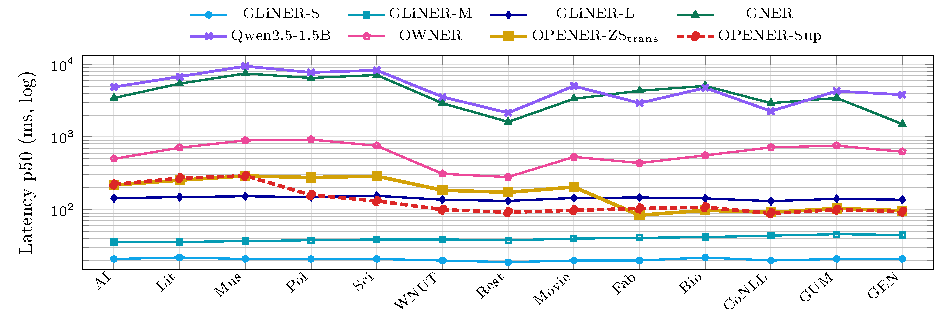
\includegraphics{Fig4}
\caption{Per-sentence inference latency (p50, ms, \emph{log} scale) per dataset (\autoref{tab:latency}). Same systems and styling as \autoref{fig:main}. OPENER-Sup is the dashed red line. The OPENER variants track GLiNER-L, while GNER and the Qwen LLM are one to two orders of magnitude slower}
\label{fig:latency}
\par\bigskip
\tablecaptype
\centering
\caption{Energy consumption per run (Wh, $\downarrow$), end-to-end.}
\label{tab:energy}
\footnotesize
\setlength{\tabcolsep}{4pt}
\begin{adjustbox}{max width=\textwidth}
\begin{threeparttable}
\begin{tabular}{l*{13}{c}c}
\toprule
Model & AI & Lit & Mus & Pol & Sci & WNUT & Rest & Movie & Fab & Bio & CoNLL & GUM & GEN & Avg \\
\midrule
\multicolumn{15}{l}{\emph{Zero-shot (no target labels)}} \\
GLiNER-S & \textbf{0.19} & \textbf{0.17} & \textbf{0.20} & \textbf{0.27} & \textbf{0.22} & \textbf{0.27} & \textbf{0.35} & \textbf{0.39} & \textbf{0.40} & \textbf{0.42} & \textbf{0.37} & \textbf{0.41} & \textbf{0.40} & \textbf{0.31} \\
GLiNER-M & 0.31 & 0.29 & 0.33 & 0.48 & 0.40 & 0.50 & 0.66 & 0.76 & 0.77 & 0.79 & 0.69 & 0.82 & 0.75 & 0.58 \\
GLiNER-L & 0.68 & 0.67 & 0.77 & 1.04 & 0.91 & 1.01 & 1.37 & 1.51 & 1.54 & 1.49 & 1.38 & 1.52 & 1.43 & 1.18 \\
GNER & 17.13 & 24.28 & 39.75 & 50.88 & 44.76 & 20.60 & 17.02 & 37.17 & 49.11 & 63.50 & 45.22 & 38.69 & 26.50 & 36.51 \\
Qwen2.5-1.5B\textsuperscript{b} & 12.7 & 15.1 & 17.5 & 18.4 & 18.0 & 7.9 & 4.6 & 9.5 & 7.0 & 11.1 & 7.3 & 10.2 & 9.5 & 11.4 \\
OWNER\textsuperscript{c} & 6.6 & 9.0 & 12.7 & 18.3 & 12.6 & 6.5 & 8.6 & 16.3 & 13.4 & 17.1 & 22.0\textsuperscript{a} & 23.2 & 19.1 & 14.3 \\
\zsind & 0.95 & 1.06 & 1.37 & 1.97 & 1.69 & 1.52 & 2.07 & 2.28 & 2.15 & 2.30 & 2.10 & 2.33 & 2.26 & 1.85 \\
\rowcolor{hlyellow} \zstr & 1.14 & 1.23 & 1.58 & 2.08 & 1.82 & 1.41 & 1.82 & 2.23 & 1.62 & 1.87 & 1.63 & 1.90 & 1.79 & 1.70 \\
% MOVED to architecture search (\autoref{tab:ablation}); preserved e2e per-dataset:
% OPENER-ZS (transd.) & 0.97 & 1.04 & 1.36 & 1.89 & 2.04 & 2.15 & 3.15 & 2.68 & 2.08 & 1.97 & 1.48 & 1.85 & 1.90 & 1.89 \\
\addlinespace
\multicolumn{15}{l}{\emph{Supervised (target labels)}} \\
% PRESERVED pre-hard-mining OPENER energy (had a CodeCarbon glitch on Mus=22.76; avg inflated to 3.39):
% OPENER & 0.86 & 2.16 & 22.76 & 1.89 & 2.21 & 1.27 & 1.66 & 2.06 & 1.66 & 2.08 & 1.70 & 1.93 & 1.82 & 3.39 \\
\rowcolor{hlred} OPENER-Sup & 1.10 & 1.26 & 0.87 & 1.76 & 1.41 & 1.31 & 1.75 & 1.87 & 1.96 & 1.97 & 1.73 & 1.91 & 1.78 & 1.59 \\
\bottomrule
\end{tabular}
\begin{tablenotes}[flushleft]
\footnotesize
\item Abbreviations follow \autoref{tab:datasets}. Best per column in bold.
\item[a] CoNLL is its in-domain training source, measured by a separate inference-only run.
\item[b] Qwen2.5-1.5B-Instruct (4-bit) is on a $150$-sentence subsample per set.
\item[c] OWNER is measured at inference only (its one-time $88$-min CoNLL-2003 training is amortised, not charged per run).
\end{tablenotes}
\end{threeparttable}
\end{adjustbox}
\par\bigskip
\figurecaptype
\centering
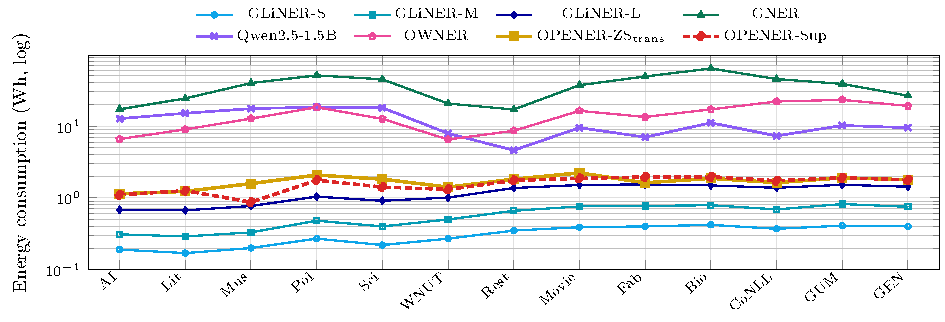
\includegraphics{Fig5}
\caption{Per-run energy consumption (Wh, \emph{log} scale) per dataset (\autoref{tab:energy}). Same systems and styling as \autoref{fig:main}. The OPENER variants sit an order of magnitude below OWNER and the generative GNER/Qwen baselines}
\label{fig:energy}
\end{table*}

OWNER is run in its native protocol \cite{genest2025owner}: a single model is trained once on the CoNLL-2003 source (a one-time cost of $88$ minutes on our 6\,GB GPU) and then applied \emph{zero-shot} to every target set (cells marked \textsuperscript{c}).
CoNLL-2003 is therefore in-domain for OWNER (marked \textsuperscript{a}) and is excluded when reading OWNER as a transfer system.
Concretely, excluding CoNLL-2003 (in-domain for both OWNER and OPENER), OWNER's reported $34.3$ thirteen-set mean becomes a $32.9$ transfer mean, still well below \zstr ($39.1$ on the same $12$ sets). The margin in fact widens from $+5.2$ to $+6.2$ AMI under this fair transfer reading.
One protocol asymmetry must be kept in mind when reading the typing scores: OPENER-Sup fits a lightweight linear classifier on each target's training split (a supervised probe), whereas OWNER, GLiNER and GNER use no target-side labels.
The two systems thus trade annotation for inference cost: OPENER-Sup needs target labels but stays cheap at test time, while OWNER needs none but pays a heavy per-sentence cost, it re-encodes every mention and clusters at inference time, an order of magnitude above OPENER (\autoref{tab:latency} and \autoref{fig:latency}, \autoref{tab:energy} and \autoref{fig:energy}).


To close this asymmetry, we also evaluate OPENER-ZS, a zero-shot variant that drops the supervised probe and types each mention against label-name prototypes, using no target labels.
Its un-refined nearest-centroid baseline, \zsind, already sits within half a point of the zero-shot OWNER baseline end-to-end ($33.8$ vs $34.3$ mean AMI) and matches it on gold ($43.2$ vs $43.0$, \autoref{tab:et-gold}), while keeping OPENER's frugal inference profile ($137$\,ms, $1.85$\,Wh vs $616$\,ms, $14.3$\,Wh).
Two label-free refinements then build \zstr: a transductive k-means on the prototypes, and \emph{fusing in the detector's own zero-shot label predictions}, a signal the centroid otherwise discards, which together reach $39.5$ end-to-end, the best of all compared zero-shot systems, ahead of GLiNER-L ($38.9$) and within $0.6$ AMI of OPENER-Sup, all without any target label.
For reference, the only generative LLM that fits our $6$\,GB GPU, Qwen2.5-1.5B-Instruct \cite{qwen2025} in 4-bit, prompted for JSON-formatted entities, trails every dedicated system ($26.1$ mean AMI on a $150$-sentence subsample, \autoref{tab:main}) while being the slowest per sentence ($5.1$\,s) and the most energy-hungry once normalised by sentence count ($11.4$\,Wh over only $150$ sentences, about twice GNER's per-sentence draw, \autoref{tab:efficiency} and \autoref{fig:metrics-bars}): a small open LLM pays on both axes at once.

% --- Table 8 + Fig. 6: table and figure in ONE float, so LaTeX keeps them together and in order
% ([!t] only: at the top of a page with text below, not alone on a half-empty float page)
\begin{table*}[!t]
\centering
\caption{Quality vs efficiency, $13$-set means.}
\label{tab:efficiency}
\small
\begin{adjustbox}{max width=\textwidth}
\begin{threeparttable}
\begin{tabular}{lrrrrr}
\toprule
Model & Params & AMI\,$\uparrow$ & p50 (ms)\,$\downarrow$ & Energy (Wh)\,$\downarrow$ & CO\textsubscript{2} (g)\,$\downarrow$ \\
\midrule
\multicolumn{6}{l}{\emph{Zero-shot (no target labels)}} \\
GLiNER-S  & 50M  & 36.5 & 21 & 0.31 & 0.02 \\
GLiNER-M  & 200M & 37.1 & 40 & 0.58 & 0.03 \\
GLiNER-L  & 330M & 38.9 & 143 & 1.18 & 0.07 \\
GNER      & 220M & 37.9 & 4226 & 36.51 & 2.05 \\
Qwen2.5-1.5B (4-bit)\textsuperscript{b} & 1.5B & 26.1 & 5051 & 11.4 & 0.60 \\
OWNER\textsuperscript{c} & 294M & 34.3 & 616 & 14.3 & 0.74 \\
\zsind & 467M & 33.8$_{\pm0.7}$ & 137 & 1.85 & 0.10 \\
\rowcolor{hlyellow} \zstr & 467M & 39.5$_{\pm0.1}$ & 182 & 1.70 & 0.10 \\
% MOVED to architecture search (\autoref{tab:ablation}); preserved:
% OPENER-ZS (transd.) & 467M & 36.8 & 151 & 1.89 & 0.11 \\
\addlinespace
\multicolumn{6}{l}{\emph{Supervised (target labels)}} \\
% PRESERVED pre-hard-mining: OPENER & 467M & 36.6 & 160 & 3.39 & 0.19 \\ (energy inflated by a CodeCarbon glitch on Mus)
\rowcolor{hlred} OPENER-Sup & 467M & 40.1$_{\pm0.5}$ & 143 & 1.59 & 0.09 \\
\bottomrule
\end{tabular}
\begin{tablenotes}[flushleft]
\footnotesize
\item AMI ($\times 100$, $\uparrow$, OPENER rows: mean\,$\pm$\,std over three retraining seeds). P50 latency (ms), energy (Wh), carbon (gCO\textsubscript{2}eq) per run ($\downarrow$, measured on the released seed-$42$ run). Parameters (end-to-end OPENER $=$ GLiNER-L detector $330$M $+$ embedder $137$M $=$ $467$M, or $137$M on gold, OWNER $\approx$294M, GLiNER parameter counts from the released checkpoints).
\item[b] Qwen2.5-1.5B-Instruct (4-bit) is on a $150$-sentence subsample per set.
\item[c] OWNER's latency is an amortised wall-clock mean and its one-time $88$-min training is not charged per run (\autoref{tab:latency}).
\end{tablenotes}
\end{threeparttable}
\end{adjustbox}
\par\bigskip
\figurecaptype
\centering
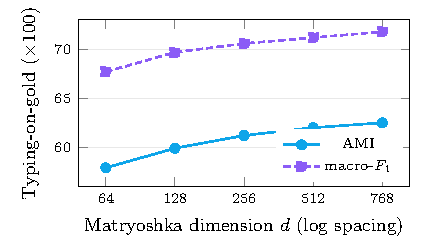
\includegraphics{Fig6}
\caption{Per-model means on the four axes ($13$-set averages, \autoref{tab:efficiency}). The light dotted line separates the \emph{zero-shot} systems (left) from the \emph{supervised} OPENER-Sup (right). Latency, energy and CO\textsubscript{2} use a log scale. Labels: GL-S/M/L $=$ GLiNER sizes, OWN $=$ OWNER, ZS$_i$ $=$ \zsind, ZS$_t$ $=$ \zstr, Sup $=$ OPENER-Sup}
\label{fig:metrics-bars}
\end{table*}

OPENER-Sup remains the stronger configuration ($40.1$ end-to-end, $62.3$ on gold), so OPENER-ZS is best read as the frugal, annotation-free operating point of the same pipeline.
A per-domain analysis of these results, the detection bottleneck and the learned embedding geometry follows in \autoref{sec:exp:analysis}.




% RESOLVED[2026-06-13]: the 22.76 Wh CodeCarbon glitch on crossner_music is gone in the
% hard-mining e2e re-run (Mus = 1.72 Wh). OPENER energy row + averages now come from that
% clean run; true mean energy is 1.88 Wh (was 3.39, inflated by the single glitched cell).



\subsection{Analysis}
\label{sec:exp:analysis}

\paragraph{Where OPENER wins, and why}
Two domain patterns stand out across \autoref{tab:main} and \autoref{fig:main}.

First, the detector-fusion gains of \zstr concentrate on the context-rich encyclopaedic CrossNER domains ($+14.7$ AMI on Music, $+10.1$ on Science, $+8.8$ on Politics over the un-fused centroid), where the detector's own zero-shot label is most reliable and lifts OPENER-ZS to detector-level quality (e.g.\ Music $58.3$, edging GLiNER-L's $58.0$).

Second, on specialised schemas with opaque, abbreviation-like labels (FabNER, BioNLP), OPENER's contrastive typing maps cryptic surface forms far better than prompt-based naming models, as OWNER: OPENER-Sup leads end-to-end ($29.8$ and $35.9$ AMI), and on gold mentions, the gap widens sharply ($57.1$/$69.2$ versus OWNER's $31.9$/$29.2$, \autoref{tab:et-gold}).


\paragraph{Detection is the bottleneck, worst on specialised domains}
Contrasting typing on gold mentions with the end-to-end scores isolates the cost of detection.
For OPENER-Sup, the mean drop from gold to end-to-end is $22.2$ AMI, but it is far from uniform: it averages $18.8$ on the encyclopaedic CrossNER domains against $29.9$ on the specialised schemas (BioNLP, MIT-Restaurant, MIT-Movie, FabNER), peaking at $33.3$ on BioNLP.
The typing head is strong everywhere (gold AMI above $50$ on $11$ of $13$ sets). What caps end-to-end quality is the open-world detector's recall on cryptic, domain-specific surface forms, which confirms detection, not typing, as the dominant bottleneck. The clearest next step for this method is therefore to build and train a stronger mention detector, which we expect to raise the end-to-end scores drastically.

\paragraph{What remains hard}
The residual typing errors are dominated by confusions between fine-grained, lexically close types within a domain rather than across domains.
The most frequent type confusions are DNA vs.\ protein (BioNLP), the FabNER process labels CONPRI vs.\ MATE/PRO/MANP, and the Movie attributes TITLE vs.\ GENRE/RATING: precisely the opaque schemas of \autoref{tab:datasets} where even the surrounding context barely disambiguates the type.

\paragraph{Contrastive learning in action}
\autoref{fig:umap} visualises the effect of the two fine-tuning stages on a \emph{held-out} domain (WNUT-17), never seen during contrastive training.
Frozen and unmodified, the Nomic embedding intermixes entity types. The contrastive step already pulls same-type mentions together, and the hard-negative mining pass sharpens the boundaries between the types it most often confuses, yielding compact, well-separated clusters.
The type geometry learned on CoNLL thus transfers to an unseen domain, which is what makes the cheap label-name and linear typing heads effective.



\subsection{Ablations}
\label{sec:exp:ablations}
We justify each architectural choice with a one-factor-at-a-time search: starting from the default pipeline, we vary a single component, hold the others fixed, and keep the setting with the highest mean AMI.
Among embedder variants, an error-driven \emph{hard-negative mining} pass, fine-tuning the contrastive embedder on the entity pairs it most often confuses (e.g.\ \emph{writer}/\emph{person}, \emph{album}/\emph{band}, \emph{country}/\emph{location}), mixed with correctly-typed mentions for diversity, raises typing-on-gold AMI from $54.0$ to $60.1$. Scaling the mined triplets ($3000\!\to\!8000$) and epochs ($2\!\to\!3$) lifts it further to $62.5$ ($+8.5$ over the contrastive embedder, better on $12$ of $13$ sets), our selected configuration.
\autoref{tab:ablation} reports this search.

\begin{table*}[!t]
\centering
\caption{OPENER architecture search: one component is varied at a time around the default pipeline (\textbf{bold}).}
\label{tab:ablation}
\small
\begin{adjustbox}{max width=\textwidth}
\begin{threeparttable}
\begin{tabular}{lccrrrr}
\toprule
Configuration & AMI\,$\uparrow$ & F\textsubscript{1}\,$\uparrow$ & Fit\,(ms)\,$\downarrow$ & p50\,(ms)\,$\downarrow$ & En.\,(Wh)\,$\downarrow$ & CO\textsubscript{2}\,(g)\,$\downarrow$ \\
\midrule
\multicolumn{7}{l}{\emph{Mention detector} (each row: that detector \,$\rightarrow$\, OPENER embedder $+$ typing head)} \\
\quad GLiNER-S                       & 37.7 & 28.8 & 0.0 & 51 & 0.73 & 0.04 \\
\quad GLiNER-M                       & 38.0 & 28.7 & 0.0 & 70 & 1.01 & 0.06 \\
\quad \textbf{GLiNER-L} (open-world) & \textbf{40.2} & \textbf{30.5} & 0.0 & 143 & 1.59 & 0.09 \\
\quad BERT-NER (closed-set) \cite{devlin2019bert}      & 33.9 & 17.9 & 0.0 & 68 & 0.58 & 0.03 \\
\quad RoBERTa-NER (closed-set) \cite{liu2019roberta}   & 39.4 & 24.6 & 0.0 & 54 & 0.58 & 0.04 \\
\addlinespace
\multicolumn{7}{l}{\emph{Entity embedder}\textsuperscript{a}} \\
\quad frozen bge-base-en-v1.5 \cite{xiao2024cpack}      & 23.6 & 41.9 & 0 & 43 & 0.63 & 0.04 \\
\quad frozen all-mpnet-base-v2 \cite{song2020mpnet}     & 24.1 & 42.6 & 0 & 52 & 0.85 & 0.05 \\
\quad frozen mxbai-embed-large-v1 \cite{li2024aoe}      & 24.4 & 42.5 & 0 & 363 & 3.86 & 0.25 \\
\quad frozen e5-base-v2 \cite{wang2022e5}               & 25.3 & 43.4 & 0 & 39 & 0.59 & 0.04 \\
\quad frozen Nomic v1.5 (selected base)                 & 25.8 & 43.9 & 0 & 42 & 0.63 & 0.04 \\
\quad + contrastive (Triplet, CoNLL, 3\,ep.)            & 54.0 & 63.3 & 0 & 42 & 0.63 & 0.04 \\
\quad + hard-negative mining (2\,ep., 3k\,tr.)          & 60.1 & 68.8 & 0 & 42 & 0.63 & 0.04 \\
\quad \textbf{+ hard-negative mining (3\,ep., 8k\,tr.)} & \textbf{62.5} & \textbf{71.8} & 0 & 42 & 0.63 & 0.04 \\
\addlinespace
\multicolumn{7}{l}{\emph{Matryoshka dimension}\textsuperscript{b}} \\
\quad 64                             & 57.9 & 67.7 & 299 & 42 & 0.63 & 0.04 \\
\quad 128                            & 59.9 & 69.7 & 562 & 42 & 0.63 & 0.04 \\
\quad 256                            & 61.2 & 70.6 & 926 & 42 & 0.63 & 0.04 \\
\quad 512                            & 62.0 & 71.2 & 1556 & 42 & 0.63 & 0.04 \\
\quad \textbf{768}                   & \textbf{62.5} & \textbf{71.8} & 2176 & 42 & 0.63 & 0.04 \\
\addlinespace
\multicolumn{7}{l}{\emph{Entity typing}\textsuperscript{c}} \\
\quad GMM (per-class)                & 56.1 & 65.3 & 527 & 42 & 0.63 & 0.04 \\
\quad LogReg                         & 55.6 & 53.5 & 546 & 42 & 0.63 & 0.04 \\
\quad LogReg (balanced)              & 57.8 & 67.5 & 485 & 42 & 0.63 & 0.04 \\
\quad LinearSVC                      & 61.7 & 66.5 & 2041 & 42 & 0.63 & 0.04 \\
\quad \textbf{LinearSVC (balanced)}  & \textbf{62.5} & \textbf{71.8} & 2217 & 42 & 0.63 & 0.04 \\
\quad Nearest centroid (zero-shot)\textsuperscript{d} & 44.4 & 46.8 & 293 & 42 & 0.63 & 0.04 \\
\quad \quad + transductive refine\textsuperscript{d} & 51.4 & 48.5 & 293 & 42 & 0.63 & 0.04 \\
\bottomrule
\end{tabular}
\begin{tablenotes}[flushleft]
\footnotesize
\item[] Metrics. AMI and macro-$F_1$ ($\times100$, $\uparrow$). Fit\,(ms) is the typing-head training time. Latency, energy and carbon are per row ($\downarrow$). All rows use the released seed ($42$).
\item[] Protocol, which differs per axis. On the \emph{mention-detector} axis each row is OPENER's \emph{end-to-end} AMI with that detector, which only proposes spans that the OPENER head re-types (unlike the standalone systems of \autoref{tab:main}). The \textsuperscript{a}\,embedder, \textsuperscript{c}\,typing and \textsuperscript{b}\,dimension axes are instead \emph{typing-on-gold} over the $13$ sets.
\item[] Cost. Latency and energy are the deployed end-to-end cost on the mention-detector axis, and the constant embedder-plus-typing cost on the other axes.
\item[b] Truncates the Matryoshka vector after encoding.
\item[d] Zero-shot nearest-centroid head (no target labels). Its Fit is the one-off prototype-embedding cost.
\end{tablenotes}
\end{threeparttable}
\end{adjustbox}
\end{table*}
The remaining axes confirm the rest of the pipeline: among frozen ready-to-use base encoders, Nomic v1.5 is the most discriminative for entity typing ($25.8$ AMI, ahead of e5-base $25.3$, mxbai $24.4$, MPNet $24.1$ and BGE $23.6$) and is selected (the heaviest candidate, mxbai-large, is moreover $\sim$8$\times$ slower per sentence for no quality gain). Even so, frozen embeddings are only weakly discriminative, so the contrastive step is what makes the space usable ($+28.2$). The detector trades quality for cost (GLiNER-S\,$\to$\,L: $37.7\!\to\!40.2$ AMI at $51\!\to\!143$\,ms end-to-end), and OPENER's typing on GLiNER-L's spans ($40.2$) even beats GLiNER-L's own typing ($38.9$, \autoref{tab:main}). A closed-set NER detector (BERT or RoBERTa-NER, CoNLL-trained) used in its place collapses to $\sim$0 recall outside PER/ORG/LOC/MISC (MIT, FabNER, BioNLP), dragging macro-$F_1$ to $17.9$/$24.6$ (vs $30.5$) and confirming that open-world detection is required. And for typing a balanced linear SVM edges out a per-class GMM and logistic regression ($62.5$ vs $56.1$ vs $55.6$).
Replacing the supervised typing head with a label-name nearest-centroid removes target supervision entirely, at a cost of $18.1$ AMI ($62.5\!\to\!44.4$). This base variant, \zsind, stays on par with the zero-shot OWNER baseline ($43.2$ vs $43.0$ over the three seeds, \autoref{tab:et-gold}) while fitting in $293$\,ms instead of $2.2$\,s, making it the frugal choice when no target labels are available.
A label-free \emph{transductive} refinement of the prototypes, spherical k-means seeded by the label names and run once on the unlabelled test mentions, recovers $7.0$ AMI on gold mentions ($44.4\!\to\!51.4$, \autoref{tab:ablation}) and $2.6$ end-to-end at the released seed ($34.2\!\to\!36.8$, above OWNER's $34.3$), widening \zstr's margin over OWNER while still using no target labels. This is a transductive rather than inductive setting, as it exploits the unlabelled test distribution.
We further probed whether the zero-shot head could be improved by aligning entity mentions and label names in a shared space, trained on the large label vocabulary of Pile-NER \cite{zhou2024universalner} ($\approx$4.6k types, \autoref{tab:zs-embedder}).
Although strictly domain-agnostic, since it never sees any target-side data, it does not improve mean AMI ($42.2$ vs $44.4$), and a second label-name hard-mining pass degrades it further ($39.7$) because Pile-NER's GPT-generated types contain many near-synonyms (e.g.\ \emph{person}/\emph{per}, \emph{location}/\emph{loc}) whose mined ``confusions'' pull apart labels that should stay close.
We therefore retain the target-tuned embedder for OPENER-ZS and report the Pile-NER variants as a negative ablation.

A separate efficiency axis emerges in the \emph{training} cost (\autoref{tab:ablation}, Fit): per-sentence inference is governed by the detector alone (truncating the Matryoshka dimension or swapping the classifier leaves it unchanged), whereas fitting the typing head is $7\times$ cheaper at dimension $64$ than at $768$ (for only a $4.6$-point AMI drop, $62.5\!\to\!57.9$) and $4.5\times$ cheaper for balanced logistic regression than for the linear SVM, a speed/quality knob orthogonal to inference.
To isolate the entity-typing component itself, \autoref{tab:et-gold} compares OPENER against OWNER on gold mentions, where detection errors are removed.
One cell stands out: \zsind drops to $16.1$ AMI on MIT-Movie, with the largest seed variance of the table ($\pm 7.1$), which we attribute to attribute-like label names (PLOT, REVIEW, TRAILER) carrying little lexical signal in a corpus where every mention is movie-related, leaving the prototypes poorly anchored. The transductive refinement of \zstr recovers most of this gap ($44.8$).
The higher end-to-end value of \zsind on the same set ($32.8$, \autoref{tab:main}) does not contradict the gold score: the sentinel labels added by the end-to-end protocol reshape both partitions, so the two AMI values are not directly comparable.

\begin{table*}[!t]
\centering
\caption{Entity typing on gold mentions (detection bypassed): OPENER vs OWNER (AMI $\times 100$, $\uparrow$).}
\label{tab:et-gold}
\scriptsize
\setlength{\tabcolsep}{2.5pt}
\begin{adjustbox}{max width=\textwidth}
\begin{threeparttable}
\begin{tabular}{l*{13}{c}c}
\toprule
Model & AI & Lit & Mus & Pol & Sci & WNUT & Rest & Movie & Fab & Bio & CoNLL & GUM & GEN & Avg \\
\midrule
%       --       DATA PRESERVED (pre-hard-mining OPENER, contrastive only, 2026-06-11)       --
% OWNER\textsuperscript{c} & \textbf{55.7} & \textbf{54.3} & 59.8 & 63.2 & 63.1 & 30.5 & 29.3 & 31.8 & 31.9 & 29.2 & 52.5\textsuperscript{a} & 30.0 & 27.2 & 43.0 \\
% OPENER & 55.6 & 53.5 & \textbf{64.2} & \textbf{66.6} & \textbf{66.1} & \textbf{41.8} & \textbf{51.2} & \textbf{54.2} & \textbf{36.5} & \textbf{60.2} & \textbf{70.7} & \textbf{37.7} & \textbf{44.2} & \textbf{54.0} \\
%       --       end preserved       --
\multicolumn{15}{l}{\emph{Zero-shot (no target labels)}} \\
OWNER & 55.7 & 54.3 & 59.8 & 63.2 & 63.1 & 30.5 & 29.3 & 31.8 & 31.9 & 29.2 & 52.5\textsuperscript{a} & 30.0 & 27.2 & 43.0 \\
\zsind & 38.7$_{\pm3.6}$ & 57.7$_{\pm3.3}$ & 54.7$_{\pm1.7}$ & 57.4$_{\pm5.8}$ & 57.8$_{\pm1.6}$ & 31.3$_{\pm2.6}$ & 38.1$_{\pm4.6}$ & 16.1$_{\pm7.1}$ & 30.4$_{\pm5.1}$ & 51.1$_{\pm2.9}$ & 63.9$_{\pm3.0}^{\text{a}}$ & 33.7$_{\pm3.8}$ & 31.0$_{\pm2.5}$ & 43.2$_{\pm1.3}$ \\
\rowcolor{hlyellow} \zstr & 46.1$_{\pm2.0}$ & 63.5$_{\pm2.3}$ & 67.0$_{\pm1.9}$ & 66.4$_{\pm1.2}$ & 59.6$_{\pm2.0}$ & 32.7$_{\pm2.8}$ & 47.3$_{\pm4.8}$ & 44.8$_{\pm1.1}$ & 33.9$_{\pm3.3}$ & 49.8$_{\pm0.3}$ & 70.7$_{\pm1.7}^{\text{a}}$ & 41.5$_{\pm2.5}$ & 38.8$_{\pm1.6}$ & 50.9$_{\pm0.4}$ \\
\addlinespace
\multicolumn{15}{l}{\emph{Supervised (target labels)}} \\
% hard-mining 3k tr./2 ep. (recorded in project notes): 57.3 64.7 71.1 72.5 67.2 40.1 59.5 61.1 50.7 64.7 70.6 48.6 53.1 | 60.1
\rowcolor{hlred} OPENER-Sup & \textbf{57.6$_{\pm0.9}$} & \textbf{66.0$_{\pm2.0}$} & \textbf{72.3$_{\pm1.5}$} & \textbf{73.6$_{\pm1.8}$} & \textbf{69.4$_{\pm2.2}$} & \textbf{38.8$_{\pm1.0}$} & \textbf{63.2$_{\pm2.0}$} & \textbf{67.7$_{\pm1.9}$} & \textbf{57.1$_{\pm2.0}$} & \textbf{69.2$_{\pm1.8}$} & 73.3$_{\pm1.6}^{\text{a}}$ & \textbf{49.8$_{\pm0.6}$} & \textbf{51.5$_{\pm0.2}$} & \textbf{62.3$_{\pm1.0}$} \\
\bottomrule
\end{tabular}
\begin{tablenotes}[flushleft]
\footnotesize
\item[] Reading. Abbreviations follow \autoref{tab:datasets}. Bold marks the best value per column. Systems are grouped by supervision.
\item[] Statistics. OPENER rows report mean\,$\pm$\,std over the three embedder-retraining seeds (\autoref{sec:exp:protocol}). OWNER is a single training run.
\item[] Typing heads. \zsind is the un-refined nearest centroid and \zstr adds the transductive refinement. Note that the detector fusion of \autoref{tab:main} is end-to-end-only, so it is inactive here, where detection is bypassed. OPENER-Sup is the supervised upper bound.
\item[] Outlier. The low \zsind MIT-Movie cell ($16.1 \pm 7.1$) is analysed in \autoref{sec:exp:ablations}: the schema's attribute-like label names give the prototypes little lexical signal, and the sentinel-based end-to-end score of \autoref{tab:main} is not directly comparable to this gold score.
\item[a] CoNLL-2003 is in-domain for OWNER (training source) and OPENER (contrastive source) and is not bolded.
\end{tablenotes}
\end{threeparttable}
\end{adjustbox}
\end{table*}
\begin{table*}[!t]
\centering
\caption{Zero-shot typing: effect of the contrastive embedder on \zsind (typing-on-gold, $13$-set means at the released seed ($42$)).}
\label{tab:zs-embedder}
\small
\begin{adjustbox}{max width=\textwidth}
\begin{threeparttable}
\begin{tabular}{llccc}
\toprule
Embedder & Training data & AMI & F\textsubscript{1} & Acc \\
\midrule
hard-neg.\ mining (selected) & CoNLL + targets' train & \textbf{44.4} & 46.8 & 53.6 \\
Pile-NER (entity$\leftrightarrow$label) & Pile-NER only & 42.2 & \textbf{50.6} & \textbf{53.9} \\
\quad + label-name hard mining & Pile-NER only & 39.7 & 41.4 & 44.7 \\
\bottomrule
\end{tabular}
\begin{tablenotes}[flushleft]
\footnotesize
\item The nearest label-name centroid head is fixed, only the embedder changes. AMI, macro-$F_1$, accuracy ($\times100$, $\uparrow$). Best per column in bold. The selected hard-negative-mining embedder (target-tuned) is compared with Pile-NER \cite{zhou2024universalner} variants that are strictly domain-agnostic (never see target data). We report Pile-NER as a negative ablation (\autoref{sec:exp:ablations}).
\end{tablenotes}
\end{threeparttable}
\end{adjustbox}
\end{table*}


\autoref{fig:matryoshka} plots typing-on-gold quality against the Matryoshka dimension $d$. Quality degrades smoothly as $d$ shrinks, with clearly diminishing returns rather than a cliff: $d{=}256$ already reaches $61.2$ AMI (within $1.3$ of the full $62.5$) and the curve flattens above it. Truncation therefore trades a little quality for a large cut in the typing-head fit cost, and, crucially, this confirms that the Matryoshka structure \emph{survives} our contrastive fine-tuning: the embedder can still be truncated and renormalised, exposing a graceful cost/quality knob.

\begin{figure}[!t]
\centering
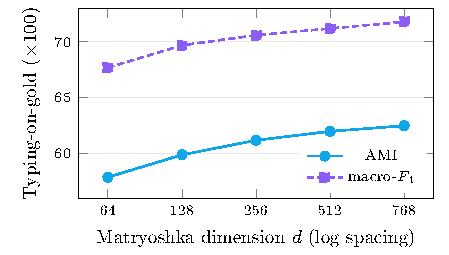
\includegraphics[width=\linewidth]{Fig7}
\caption{Typing-on-gold quality vs the Matryoshka truncation dimension $d$. Both AMI and macro-$F_1$ degrade smoothly, with diminishing returns rather than a cliff, and flatten above $d{=}256$. Truncation is therefore a graceful cost/quality knob, and the Matryoshka structure survives the contrastive fine-tuning. Data from \autoref{tab:ablation} (dimension axis, released seed, $13$-set means, log-spaced $d$)}
\label{fig:matryoshka}
\end{figure}



% (per-dataset end-to-end line chart is placed next to tab:main as fig:main)

%       --       RAW per-dataset AMI x100 (OPENER-ZS gold), order AI..GEN, preserved 2026-06-14       --
% hard_big (selected) : 41.4 61.4 55.2 50.7 58.0 33.0 42.6 18.4 35.6 54.1 65.9 31.1 30.2 | 44.4
% pilener BASE        : 48.8 52.9 58.2 64.9 66.6 38.3 26.8  9.5 23.8 42.2 50.4 30.7 35.2 | 42.2
% pilener HARD        : (mean 39.7 / F1 41.4 / acc 44.7) ; e2e pilener HARD mean AMI 33.9 vs hard_big 34.2
% Results dirs: outputs/results/opener_zs_pilener{,_hard,_hard_e2e}/ ; embedders: outputs/models/embedder_pilener{,_hard}/
%       --       end raw       --

% No \FloatBarrier here: in the two-column layout it forced Tables 10 and 11 out
% before the Conclusion and left half of the previous page blank.



% (note FR remplacée par le paragraphe Matryoshka + Fig. matryoshka dans l'analyse des ablations)

\section{Conclusion}
\label{sec:conclusion}

We presented OPENER, an open-world NER pipeline assembled entirely from ready-to-use components, a frozen detector, a pretrained Matryoshka embedder sharpened by a light contrastive fine-tuning with error-driven hard-negative mining, and a swappable typing head, with no encoder trained from scratch.
The modular design is part of the result rather than an implementation detail. Because the three stages are independently swappable, we could search the architecture one axis at a time (\autoref{tab:ablation}) and select every component on measured evidence instead of by assumption, and the same modularity keeps the embedder's Matryoshka structure usable as a compute/quality knob even after our contrastive fine-tuning (\autoref{fig:matryoshka}).

Both operating points of the typing head perform strongly, at opposite ends of the supervision axis.
Our zero-shot head OPENER-ZS, label-name prototypes refined transductively and fused with the detector's own predictions, needs no target labels at typing time and is still the best of the compared zero-shot systems end-to-end ($39.5$ AMI, all AMI scores being reported $\times 100$ as in the tables), ahead of GLiNER-L, GNER, Qwen2.5 and OWNER, at one to two orders of magnitude lower energy than the trained-encoder and generative baselines.
When a domain's entity classes are fixed and labelled, a balanced linear probe, OPENER-Sup, goes further. On gold mentions, the contrastive space is highly discriminative, and OPENER-Sup is the most accurate system in our benchmark, leading on all $13$ sets and surpassing a zero-shot transfer of OWNER ($62.3$ vs $43.0$ AMI). It also attains the best end-to-end AMI of the compared systems ($40.1$ AMI*100).

Both results rest on a benchmark that is itself a contribution: $13$ open-world NER datasets on which quality, per-sentence latency and energy are reported jointly, typing-on-gold is kept separate from end-to-end, and the supervision asymmetry between systems is stated rather than hidden. Every OPENER number is averaged over three full embedder-retraining seeds.

Two findings carry beyond the specific system.
First, an open-world typing head need not train its own encoder: a general-purpose embedding, once sharpened by a light contrastive step, is already discriminative enough to type entities, and the cost that does matter is fitting the cheap typing head, not the embedder.
Second, the three-axis evaluation locates the open-world bottleneck in \emph{detection} rather than typing: typing on gold mentions reaches $62.3$ AMI but end-to-end scores drop to $40.1$ as detector recall falls on specialised domains. So, improving the detector, not the typing head, is the clearest axis for future gains. The evaluation also exposes efficiency gaps that an accuracy-only comparison would hide.

The approach has clear limits.
End-to-end quality is capped by detector recall on specialised domains, the shared bottleneck, not by the typing head.
Supervised typing needs target-domain labels, and while OPENER-ZS removes them at typing time it depends on the quality of the label names and, in its transductive form, on access to the unlabelled test mentions. The inductive zero-shot head is correspondingly weaker.
Finally, our experiments run on deliberately modest hardware: a single consumer GPU with $6$\,GB of VRAM, subject to thermal throttling.
This is the very setting that makes OPENER deployable, but it also bounded our experimental budget: despite an already broad benchmark ($13$ datasets, three axes and extensive ablations), we cap each test split at $1000$ sentences.
The quality scores themselves are nonetheless well characterised: retraining the full embedder under three seeds leaves the benchmark means nearly unchanged (std of $0.1$ to $1.3$ AMI on the thirteen-set means, \autoref{sec:exp:protocol}), inference is deterministic at a fixed seed, and a test-set bootstrap confirms per-dataset stability (bootstrap std of at most $1.5$ AMI, \autoref{tab:bootstrap}). Only latency and energy fluctuate ($\pm 15\%$) and are therefore read as averages rather than precise points.

Future work includes improving mention detection on specialised domains to lift the end-to-end ceiling and extending the decoupled detect-then-type design beyond NER to entity linking and relation extraction.

\backmatter

% --- JIIS: "Statements and Declarations" before the reference list ---
\section*{Statements and Declarations}
\label{sec:declarations}

\bmhead{Funding}
This research did not receive any specific grant from funding agencies in the public, commercial, or not-for-profit sectors.

\bmhead{Competing interests}
The authors declare no known competing financial interests or personal relationships that could have appeared to influence the work reported in this paper.

\bmhead{Ethics approval and consent to participate}
Not applicable.

\bmhead{Consent for publication}
Not applicable.

\bmhead{Data availability}
\label{sec:data}
All datasets used in this study are publicly available benchmarks, cited in \autoref{sec:exp:datasets}.

\bmhead{Code availability}
The code and the per-experiment configurations are openly available on GitHub (\url{https://github.com/Thibault-GAREL/LyRIDS_OPENER}), and the fine-tuned embedders of OPENER-ZS and OPENER-Sup are available on Hugging Face (\url{https://huggingface.co/Thibault-GAREL/opener-zs} and \url{https://huggingface.co/Thibault-GAREL/opener-sup}).

\bmhead{Author contributions}
\label{sec:credit}
\textbf{Thibault Garel:} Conceptualization, Methodology, Software, Investigation, Data curation, Formal analysis, Resources, Validation,  Writing (original draft), Writing (review \& editing), Visualization.
\textbf{Faiza Belbachir:} Supervision.
\textbf{Assia Soukane:} Supervision.

% --- Bibliography (sn-basic, numbered). references.bib is a synced copy of
% ../references.bib, placed here because JIIS forbids subfolders.
\bibliography{references}

\end{document}
